\documentclass[twoside,11pt]{article}
\usepackage{jair, rawfonts}
% \usepackage{jair, theapa, rawfonts}
\usepackage[backend=biber, style=apa]{biblatex}
\addbibresource{references.bib}

% OURS
% \usepackage{caption}
\usepackage{graphicx}
% \graphicspath{figures/}
\usepackage{hyperref}
\usepackage{color}
\usepackage{epigraph}
\usepackage{csquotes}
\usepackage{amssymb}
\usepackage{amsmath}
\usepackage{amsthm}
\usepackage{bbm}
\usepackage{tikz}
\usetikzlibrary{arrows}
\usetikzlibrary{shapes.geometric}
\usepackage{caption}
\usepackage{subcaption}
\usepackage[algo2e,ruled,linesnumbered,noend]{algorithm2e}
\usepackage{soul}
\usepackage{bbm}
\usepackage{eurosym}
\usepackage{booktabs}
\usepackage{float}
\theoremstyle{plain}
\newtheorem{theorem}{Theorem}
\newtheorem{corollary}[theorem]{Corollary}
\theoremstyle{definition}
\newtheorem{definition}{Definition}[section]
\newtheorem{remark}{Remark}[section]
\newtheorem{proposition}{Proposition}[section]
\newtheorem{example}{Example}[section]

% JAIR arguments
\jairheading{82}{2025}{2279-2323}{12/2024}{04/2025}
\ShortHeadings{Counterfactual Situation Testing}{Alvarez \& Ruggieri}
\firstpageno{2279}

%%
\begin{document}

%%
\title{Counterfactual Situation Testing: \\ From Single to Multidimensional Discrimination}

%%
\author{\name Jose M. Alvarez \email josemanuel.alvarez@kuleuven.be \\
\addr Department of Computer Science, KU Leuven \\ 3001 Leuven, Belgium
\AND
\name Salvatore Ruggieri \email salvatore.ruggieri@unipi.it \\
\addr Department of Computer Science, University of Pisa \\ 56126 Pisa, Italy}

%%
\maketitle

%%
\begin{abstract}
    As machine learning models enable decisions once performed only by humans, it is central to develop tools that assess the fairness of such models. Notably, within high-stake settings like hiring and lending, these tools must be able to detect potentially discriminatory models. We present counterfactual situation testing (CST), a causal data mining framework for detecting individual discrimination in a dataset of classifier decisions. CST answers the question ``what would have been the model outcome had the individual, or complainant, been of a different protected status?'' It extends the legally-grounded situation testing (ST) of \textcite{Thanh_KnnSituationTesting2011} by operationalizing the notion of \textit{fairness given the difference} via counterfactual reasoning. ST finds for each complainant similar protected and non-protected instances in the dataset; constructs, respectively, a control and test group; and compares the groups such that a difference in model outcomes implies a potential case of individual discrimination. CST, instead, avoids this idealized comparison by establishing the test group on the complainant's generated counterfactual, which reflects how the protected attribute when changed influences other seemingly neutral attributes of the complainant. Under CST we test for discrimination for each complainant by comparing similar individuals within the control and test group but dissimilar individuals across these groups. We consider single (e.g.,~gender) and multidimensional (e.g.,~gender and race) discrimination testing. For multidimensional discrimination we study multiple and intersectional discrimination and, as feared by legal scholars, find evidence that the former fails to account for the latter kind. Using a k-nearest neighbor implementation, we showcase CST on synthetic and real data. Experimental results show that CST uncovers a higher number of cases than ST, even when the model is counterfactually fair. CST, in fact, extends counterfactual fairness (CF) of \textcite{Kusner2017CF} by equipping CF with confidence intervals, which we report for all experiments.
\end{abstract}

\section{Introduction}
\label{sec:Introduction}
\section{Introduction}

% \textcolor{red}{Still on working}

% \textcolor{red}{add label for each section}


Robot learning relies on diverse and high-quality data to learn complex behaviors \cite{aldaco2024aloha, wang2024dexcap}.
Recent studies highlight that models trained on datasets with greater complexity and variation in the domain tend to generalize more effectively across broader scenarios \cite{mann2020language, radford2021learning, gao2024efficient}.
% However, creating such diverse datasets in the real world presents significant challenges.
% Modifying physical environments and adjusting robot hardware settings require considerable time, effort, and financial resources.
% In contrast, simulation environments offer a flexible and efficient alternative.
% Simulations allow for the creation and modification of digital environments with a wide range of object shapes, weights, materials, lighting, textures, friction coefficients, and so on to incorporate domain randomization,
% which helps improve the robustness of models when deployed in real-world conditions.
% These environments can be easily adjusted and reset, enabling faster iterations and data collection.
% Additionally, simulations provide the ability to consistently reproduce scenarios, which is essential for benchmarking and model evaluation.
% Another advantage of simulations is their flexibility in sensor integration. Sensors such as cameras, LiDARs, and tactile sensors can be added or repositioned without the physical limitations present in real-world setups. Simulations also eliminate the risk of damaging expensive hardware during edge-case experiments, making them an ideal platform for testing rare or dangerous scenarios that are impractical to explore in real life.
By leveraging immersive perspectives and interactions, Extended Reality\footnote{Extended Reality is an umbrella term to refer to Augmented Reality, Mixed Reality, and Virtual Reality \cite{wikipediaExtendedReality}}
(XR)
is a promising candidate for efficient and intuitive large scale data collection \cite{jiang2024comprehensive, arcade}
% With the demand for collecting data, XR provides a promising approach for humans to teach robots by offering users an immersive experience.
in simulation \cite{jiang2024comprehensive, arcade, dexhub-park} and real-world scenarios \cite{openteach, opentelevision}.
However, reusing and reproducing current XR approaches for robot data collection for new settings and scenarios is complicated and requires significant effort.
% are difficult to reuse and reproduce system makes it hard to reuse and reproduce in another data collection pipeline.
This bottleneck arises from three main limitations of current XR data collection and interaction frameworks: \textit{asset limitation}, \textit{simulator limitation}, and \textit{device limitation}.
% \textcolor{red}{ASSIGN THESE CITATION PROPERLY:}
% \textcolor{red}{list them by time order???}
% of collecting data by using XR have three main limitations.
Current approaches suffering from \textit{asset limitation} \cite{arclfd, jiang2024comprehensive, arcade, george2025openvr, vicarios}
% Firstly, recent works \cite{jiang2024comprehensive, arcade, dexhub-park}
can only use predefined robot models and task scenes. Configuring new tasks requires significant effort, since each new object or model must be specifically integrated into the XR application.
% and it takes too much effort to configure new tasks in their systems since they cannot spawn arbitrary models in the XR application.
The vast majority of application are developed for specific simulators or real-world scenarios. This \textit{simulator limitation} \cite{mosbach2022accelerating, lipton2017baxter, dexhub-park, arcade}
% Secondly, existing systems are limited to a single simulation platform or real-world scenarios.
significantly reduces reusability and makes adaptation to new simulation platforms challenging.
Additionally, most current XR frameworks are designed for a specific version of a single XR headset, leading to a \textit{device limitation} 
\cite{lipton2017baxter, armada, openteach, meng2023virtual}.
% and there is no work working on the extendability of transferring to a new headsets as far as we know.
To the best of our knowledge, no existing work has explored the extensibility or transferability of their framework to different headsets.
These limitations hamper reproducibility and broader contributions of XR based data collection and interaction to the research community.
% as each research group typically has its own data collection pipeline.
% In addition to these main limitations, existing XR systems are not well suited for managing multiple robot systems,
% as they are often designed for single-operator use.

In addition to these main limitations, existing XR systems are often designed for single-operator use, prohibiting collaborative data collection.
At the same time, controlling multiple robots at once can be very difficult for a single operator,
making data collection in multi-robot scenarios particularly challenging \cite{orun2019effect}.
Although there are some works using collaborative data collection in the context of tele-operation \cite{tung2021learning, Qin2023AnyTeleopAG},
there is no XR-based data collection system supporting collaborative data collection.
This limitation highlights the need for more advanced XR solutions that can better support multi-robot and multi-user scenarios.
% \textcolor{red}{more papers about collaborative data collection}

To address all of these issues, we propose \textbf{IRIS},
an \textbf{I}mmersive \textbf{R}obot \textbf{I}nteraction \textbf{S}ystem.
This general system supports various simulators, benchmarks and real-world scenarios.
It is easily extensible to new simulators and XR headsets.
IRIS achieves generalization across six dimensions:
% \begin{itemize}
%     \item \textit{Cross-scene} : diverse object models;
%     \item \textit{Cross-embodiment}: diverse robot models;
%     \item \textit{Cross-simulator}: 
%     \item \textit{Cross-reality}: fd
%     \item \textit{Cross-platform}: fd
%     \item \textit{Cross-users}: fd
% \end{itemize}
\textbf{Cross-Scene}, \textbf{Cross-Embodiment}, \textbf{Cross-Simulator}, \textbf{Cross-Reality}, \textbf{Cross-Platform}, and \textbf{Cross-User}.

\textbf{Cross-Scene} and \textbf{Cross-Embodiment} allow the system to handle arbitrary objects and robots in the simulation,
eliminating restrictions about predefined models in XR applications.
IRIS achieves these generalizations by introducing a unified scene specification, representing all objects,
including robots, as data structures with meshes, materials, and textures.
The unified scene specification is transmitted to the XR application to create and visualize an identical scene.
By treating robots as standard objects, the system simplifies XR integration,
allowing researchers to work with various robots without special robot-specific configurations.
\textbf{Cross-Simulator} ensures compatibility with various simulation engines.
IRIS simplifies adaptation by parsing simulated scenes into the unified scene specification, eliminating the need for XR application modifications when switching simulators.
New simulators can be integrated by creating a parser to convert their scenes into the unified format.
This flexibility is demonstrated by IRIS’ support for Mujoco \cite{todorov2012mujoco}, IsaacSim \cite{mittal2023orbit}, CoppeliaSim \cite{coppeliaSim}, and even the recent Genesis \cite{Genesis} simulator.
\textbf{Cross-Reality} enables the system to function seamlessly in both virtual simulations and real-world applications.
IRIS enables real-world data collection through camera-based point cloud visualization.
\textbf{Cross-Platform} allows for compatibility across various XR devices.
Since XR device APIs differ significantly, making a single codebase impractical, IRIS XR application decouples its modules to maximize code reuse.
This application, developed by Unity \cite{unity3dUnityManual}, separates scene visualization and interaction, allowing developers to integrate new headsets by reusing the visualization code and only implementing input handling for hand, head, and motion controller tracking.
IRIS provides an implementation of the XR application in the Unity framework, allowing for a straightforward deployment to any device that supports Unity. 
So far, IRIS was successfully deployed to the Meta Quest 3 and HoloLens 2.
Finally, the \textbf{Cross-User} ability allows multiple users to interact within a shared scene.
IRIS achieves this ability by introducing a protocol to establish the communication between multiple XR headsets and the simulation or real-world scenarios.
Additionally, IRIS leverages spatial anchors to support the alignment of virtual scenes from all deployed XR headsets.
% To make an seamless user experience for robot learning data collection,
% IRIS also tested in three different robot control interface
% Furthermore, to demonstrate the extensibility of our approach, we have implemented a robot-world pipeline for real robot data collection, ensuring that the system can be used in both simulated and real-world environments.
The Immersive Robot Interaction System makes the following contributions\\
\textbf{(1) A unified scene specification} that is compatible with multiple robot simulators. It enables various XR headsets to visualize and interact with simulated objects and robots, providing an immersive experience while ensuring straightforward reusability and reproducibility.\\
\textbf{(2) A collaborative data collection framework} designed for XR environments. The framework facilitates enhanced robot data acquisition.\\
\textbf{(3) A user study} demonstrating that IRIS significantly improves data collection efficiency and intuitiveness compared to the LIBERO baseline.

% \begin{table*}[t]
%     \centering
%     \begin{tabular}{lccccccc}
%         \toprule
%         & \makecell{Physical\\Interaction}
%         & \makecell{XR\\Enabled}
%         & \makecell{Free\\View}
%         & \makecell{Multiple\\Robots}
%         & \makecell{Robot\\Control}
%         % Force Feedback???
%         & \makecell{Soft Object\\Supported}
%         & \makecell{Collaborative\\Data} \\
%         \midrule
%         ARC-LfD \cite{arclfd}                              & Real        & \cmark & \xmark & \xmark & Joint              & \xmark & \xmark \\
%         DART \cite{dexhub-park}                            & Sim         & \cmark & \cmark & \cmark & Cartesian          & \xmark & \xmark \\
%         \citet{jiang2024comprehensive}                     & Sim         & \cmark & \xmark & \xmark & Joint \& Cartesian & \xmark & \xmark \\
%         \citet{mosbach2022accelerating}                    & Sim         & \cmark & \cmark & \xmark & Cartesian          & \xmark & \xmark \\
%         ARCADE \cite{arcade}                               & Real        & \cmark & \cmark & \xmark & Cartesian          & \xmark & \xmark \\
%         Holo-Dex \cite{holodex}                            & Real        & \cmark & \xmark & \cmark & Cartesian          & \cmark & \xmark \\
%         ARMADA \cite{armada}                               & Real        & \cmark & \xmark & \cmark & Cartesian          & \cmark & \xmark \\
%         Open-TeleVision \cite{opentelevision}              & Real        & \cmark & \cmark & \cmark & Cartesian          & \cmark & \xmark \\
%         OPEN TEACH \cite{openteach}                        & Real        & \cmark & \xmark & \cmark & Cartesian          & \cmark & \cmark \\
%         GELLO \cite{wu2023gello}                           & Real        & \xmark & \cmark & \cmark & Joint              & \cmark & \xmark \\
%         DexCap \cite{wang2024dexcap}                       & Real        & \xmark & \cmark & \xmark & Cartesian          & \cmark & \xmark \\
%         AnyTeleop \cite{Qin2023AnyTeleopAG}                & Real        & \xmark & \xmark & \cmark & Cartesian          & \cmark & \cmark \\
%         Vicarios \cite{vicarios}                           & Real        & \cmark & \xmark & \xmark & Cartesian          & \cmark & \xmark \\     
%         Augmented Visual Cues \cite{augmentedvisualcues}   & Real        & \cmark & \cmark & \xmark & Cartesian          & \xmark & \xmark \\ 
%         \citet{wang2024robotic}                            & Real        & \cmark & \cmark & \xmark & Cartesian          & \cmark & \xmark \\
%         Bunny-VisionPro \cite{bunnyvisionpro}              & Real        & \cmark & \cmark & \cmark & Cartesian          & \cmark & \xmark \\
%         IMMERTWIN \cite{immertwin}                         & Real        & \cmark & \cmark & \cmark & Cartesian          & \xmark & \xmark \\
%         \citet{meng2023virtual}                            & Sim \& Real & \cmark & \cmark & \xmark & Cartesian          & \xmark & \xmark \\
%         Shared Control Framework \cite{sharedctlframework} & Real        & \cmark & \cmark & \cmark & Cartesian          & \xmark & \xmark \\
%         OpenVR \cite{openvr}                               & Real        & \cmark & \cmark & \xmark & Cartesian          & \xmark & \xmark \\
%         \citet{digitaltwinmr}                              & Real        & \cmark & \cmark & \xmark & Cartesian          & \cmark & \xmark \\
        
%         \midrule
%         \textbf{Ours} & Sim \& Real & \cmark & \cmark & \cmark & Joint \& Cartesian  & \cmark & \cmark \\
%         \bottomrule
%     \end{tabular}
%     \caption{This is a cross-column table with automatic line breaking.}
%     \label{tab:cross-column}
% \end{table*}

% \begin{table*}[t]
%     \centering
%     \begin{tabular}{lccccccc}
%         \toprule
%         & \makecell{Cross-Embodiment}
%         & \makecell{Cross-Scene}
%         & \makecell{Cross-Simulator}
%         & \makecell{Cross-Reality}
%         & \makecell{Cross-Platform}
%         & \makecell{Cross-User} \\
%         \midrule
%         ARC-LfD \cite{arclfd}                              & \xmark & \xmark & \xmark & \xmark & \xmark & \xmark \\
%         DART \cite{dexhub-park}                            & \cmark & \cmark & \xmark & \xmark & \xmark & \xmark \\
%         \citet{jiang2024comprehensive}                     & \xmark & \cmark & \xmark & \xmark & \xmark & \xmark \\
%         \citet{mosbach2022accelerating}                    & \xmark & \cmark & \xmark & \xmark & \xmark & \xmark \\
%         ARCADE \cite{arcade}                               & \xmark & \xmark & \xmark & \xmark & \xmark & \xmark \\
%         Holo-Dex \cite{holodex}                            & \cmark & \xmark & \xmark & \xmark & \xmark & \xmark \\
%         ARMADA \cite{armada}                               & \cmark & \xmark & \xmark & \xmark & \xmark & \xmark \\
%         Open-TeleVision \cite{opentelevision}              & \cmark & \xmark & \xmark & \xmark & \cmark & \xmark \\
%         OPEN TEACH \cite{openteach}                        & \cmark & \xmark & \xmark & \xmark & \xmark & \cmark \\
%         GELLO \cite{wu2023gello}                           & \cmark & \xmark & \xmark & \xmark & \xmark & \xmark \\
%         DexCap \cite{wang2024dexcap}                       & \xmark & \xmark & \xmark & \xmark & \xmark & \xmark \\
%         AnyTeleop \cite{Qin2023AnyTeleopAG}                & \cmark & \cmark & \cmark & \cmark & \xmark & \cmark \\
%         Vicarios \cite{vicarios}                           & \xmark & \xmark & \xmark & \xmark & \xmark & \xmark \\     
%         Augmented Visual Cues \cite{augmentedvisualcues}   & \xmark & \xmark & \xmark & \xmark & \xmark & \xmark \\ 
%         \citet{wang2024robotic}                            & \xmark & \xmark & \xmark & \xmark & \xmark & \xmark \\
%         Bunny-VisionPro \cite{bunnyvisionpro}              & \cmark & \xmark & \xmark & \xmark & \xmark & \xmark \\
%         IMMERTWIN \cite{immertwin}                         & \cmark & \xmark & \xmark & \xmark & \xmark & \xmark \\
%         \citet{meng2023virtual}                            & \xmark & \cmark & \xmark & \cmark & \xmark & \xmark \\
%         \citet{sharedctlframework}                         & \cmark & \xmark & \xmark & \xmark & \xmark & \xmark \\
%         OpenVR \cite{george2025openvr}                               & \xmark & \xmark & \xmark & \xmark & \xmark & \xmark \\
%         \citet{digitaltwinmr}                              & \xmark & \xmark & \xmark & \xmark & \xmark & \xmark \\
        
%         \midrule
%         \textbf{Ours} & \cmark & \cmark & \cmark & \cmark & \cmark & \cmark \\
%         \bottomrule
%     \end{tabular}
%     \caption{This is a cross-column table with automatic line breaking.}
% \end{table*}

% \begin{table*}[t]
%     \centering
%     \begin{tabular}{lccccccc}
%         \toprule
%         & \makecell{Cross-Scene}
%         & \makecell{Cross-Embodiment}
%         & \makecell{Cross-Simulator}
%         & \makecell{Cross-Reality}
%         & \makecell{Cross-Platform}
%         & \makecell{Cross-User}
%         & \makecell{Control Space} \\
%         \midrule
%         % Vicarios \cite{vicarios}                           & \xmark & \xmark & \xmark & \xmark & \xmark & \xmark \\     
%         % Augmented Visual Cues \cite{augmentedvisualcues}   & \xmark & \xmark & \xmark & \xmark & \xmark & \xmark \\ 
%         % OpenVR \cite{george2025openvr}                     & \xmark & \xmark & \xmark & \xmark & \xmark & \xmark \\
%         \citet{digitaltwinmr}                              & \xmark & \xmark & \xmark & \xmark & \xmark & \xmark &  \\
%         ARC-LfD \cite{arclfd}                              & \xmark & \xmark & \xmark & \xmark & \xmark & \xmark &  \\
%         \citet{sharedctlframework}                         & \cmark & \xmark & \xmark & \xmark & \xmark & \xmark &  \\
%         \citet{jiang2024comprehensive}                     & \cmark & \xmark & \xmark & \xmark & \xmark & \xmark &  \\
%         \citet{mosbach2022accelerating}                    & \cmark & \xmark & \xmark & \xmark & \xmark & \xmark & \\
%         Holo-Dex \cite{holodex}                            & \cmark & \xmark & \xmark & \xmark & \xmark & \xmark & \\
%         ARCADE \cite{arcade}                               & \cmark & \cmark & \xmark & \xmark & \xmark & \xmark & \\
%         DART \cite{dexhub-park}                            & Limited & Limited & Mujoco & Sim & Vision Pro & \xmark &  Cartesian\\
%         ARMADA \cite{armada}                               & \cmark & \cmark & \xmark & \xmark & \xmark & \xmark & \\
%         \citet{meng2023virtual}                            & \cmark & \cmark & \xmark & \cmark & \xmark & \xmark & \\
%         % GELLO \cite{wu2023gello}                           & \cmark & \xmark & \xmark & \xmark & \xmark & \xmark \\
%         % DexCap \cite{wang2024dexcap}                       & \xmark & \xmark & \xmark & \xmark & \xmark & \xmark \\
%         % AnyTeleop \cite{Qin2023AnyTeleopAG}                & \cmark & \cmark & \cmark & \cmark & \xmark & \cmark \\
%         % \citet{wang2024robotic}                            & \xmark & \xmark & \xmark & \xmark & \xmark & \xmark \\
%         Bunny-VisionPro \cite{bunnyvisionpro}              & \cmark & \cmark & \xmark & \xmark & \xmark & \xmark & \\
%         IMMERTWIN \cite{immertwin}                         & \cmark & \cmark & \xmark & \xmark & \xmark & \xmark & \\
%         Open-TeleVision \cite{opentelevision}              & \cmark & \cmark & \xmark & \xmark & \cmark & \xmark & \\
%         \citet{szczurek2023multimodal}                     & \xmark & \xmark & \xmark & Real & \xmark & \cmark & \\
%         OPEN TEACH \cite{openteach}                        & \cmark & \cmark & \xmark & \xmark & \xmark & \cmark & \\
%         \midrule
%         \textbf{Ours} & \cmark & \cmark & \cmark & \cmark & \cmark & \cmark \\
%         \bottomrule
%     \end{tabular}
%     \caption{TODO, Bruce: this table can be further optimized.}
% \end{table*}

\definecolor{goodgreen}{HTML}{228833}
\definecolor{goodred}{HTML}{EE6677}
\definecolor{goodgray}{HTML}{BBBBBB}

\begin{table*}[t]
    \centering
    \begin{adjustbox}{max width=\textwidth}
    \renewcommand{\arraystretch}{1.2}    
    \begin{tabular}{lccccccc}
        \toprule
        & \makecell{Cross-Scene}
        & \makecell{Cross-Embodiment}
        & \makecell{Cross-Simulator}
        & \makecell{Cross-Reality}
        & \makecell{Cross-Platform}
        & \makecell{Cross-User}
        & \makecell{Control Space} \\
        \midrule
        % Vicarios \cite{vicarios}                           & \xmark & \xmark & \xmark & \xmark & \xmark & \xmark \\     
        % Augmented Visual Cues \cite{augmentedvisualcues}   & \xmark & \xmark & \xmark & \xmark & \xmark & \xmark \\ 
        % OpenVR \cite{george2025openvr}                     & \xmark & \xmark & \xmark & \xmark & \xmark & \xmark \\
        \citet{digitaltwinmr}                              & \textcolor{goodred}{Limited}     & \textcolor{goodred}{Single Robot} & \textcolor{goodred}{Unity}    & \textcolor{goodred}{Real}          & \textcolor{goodred}{Meta Quest 2} & \textcolor{goodgray}{N/A} & \textcolor{goodred}{Cartesian} \\
        ARC-LfD \cite{arclfd}                              & \textcolor{goodgray}{N/A}        & \textcolor{goodred}{Single Robot} & \textcolor{goodgray}{N/A}     & \textcolor{goodred}{Real}          & \textcolor{goodred}{HoloLens}     & \textcolor{goodgray}{N/A} & \textcolor{goodred}{Cartesian} \\
        \citet{sharedctlframework}                         & \textcolor{goodred}{Limited}     & \textcolor{goodred}{Single Robot} & \textcolor{goodgray}{N/A}     & \textcolor{goodred}{Real}          & \textcolor{goodred}{HTC Vive Pro} & \textcolor{goodgray}{N/A} & \textcolor{goodred}{Cartesian} \\
        \citet{jiang2024comprehensive}                     & \textcolor{goodred}{Limited}     & \textcolor{goodred}{Single Robot} & \textcolor{goodgray}{N/A}     & \textcolor{goodred}{Real}          & \textcolor{goodred}{HoloLens 2}   & \textcolor{goodgray}{N/A} & \textcolor{goodgreen}{Joint \& Cartesian} \\
        \citet{mosbach2022accelerating}                    & \textcolor{goodgreen}{Available} & \textcolor{goodred}{Single Robot} & \textcolor{goodred}{IsaacGym} & \textcolor{goodred}{Sim}           & \textcolor{goodred}{Vive}         & \textcolor{goodgray}{N/A} & \textcolor{goodgreen}{Joint \& Cartesian} \\
        Holo-Dex \cite{holodex}                            & \textcolor{goodgray}{N/A}        & \textcolor{goodred}{Single Robot} & \textcolor{goodgray}{N/A}     & \textcolor{goodred}{Real}          & \textcolor{goodred}{Meta Quest 2} & \textcolor{goodgray}{N/A} & \textcolor{goodred}{Joint} \\
        ARCADE \cite{arcade}                               & \textcolor{goodgray}{N/A}        & \textcolor{goodred}{Single Robot} & \textcolor{goodgray}{N/A}     & \textcolor{goodred}{Real}          & \textcolor{goodred}{HoloLens 2}   & \textcolor{goodgray}{N/A} & \textcolor{goodred}{Cartesian} \\
        DART \cite{dexhub-park}                            & \textcolor{goodred}{Limited}     & \textcolor{goodred}{Limited}      & \textcolor{goodred}{Mujoco}   & \textcolor{goodred}{Sim}           & \textcolor{goodred}{Vision Pro}   & \textcolor{goodgray}{N/A} & \textcolor{goodred}{Cartesian} \\
        ARMADA \cite{armada}                               & \textcolor{goodgray}{N/A}        & \textcolor{goodred}{Limited}      & \textcolor{goodgray}{N/A}     & \textcolor{goodred}{Real}          & \textcolor{goodred}{Vision Pro}   & \textcolor{goodgray}{N/A} & \textcolor{goodred}{Cartesian} \\
        \citet{meng2023virtual}                            & \textcolor{goodred}{Limited}     & \textcolor{goodred}{Single Robot} & \textcolor{goodred}{PhysX}   & \textcolor{goodgreen}{Sim \& Real} & \textcolor{goodred}{HoloLens 2}   & \textcolor{goodgray}{N/A} & \textcolor{goodred}{Cartesian} \\
        % GELLO \cite{wu2023gello}                           & \cmark & \xmark & \xmark & \xmark & \xmark & \xmark \\
        % DexCap \cite{wang2024dexcap}                       & \xmark & \xmark & \xmark & \xmark & \xmark & \xmark \\
        % AnyTeleop \cite{Qin2023AnyTeleopAG}                & \cmark & \cmark & \cmark & \cmark & \xmark & \cmark \\
        % \citet{wang2024robotic}                            & \xmark & \xmark & \xmark & \xmark & \xmark & \xmark \\
        Bunny-VisionPro \cite{bunnyvisionpro}              & \textcolor{goodgray}{N/A}        & \textcolor{goodred}{Single Robot} & \textcolor{goodgray}{N/A}     & \textcolor{goodred}{Real}          & \textcolor{goodred}{Vision Pro}   & \textcolor{goodgray}{N/A} & \textcolor{goodred}{Cartesian} \\
        IMMERTWIN \cite{immertwin}                         & \textcolor{goodgray}{N/A}        & \textcolor{goodred}{Limited}      & \textcolor{goodgray}{N/A}     & \textcolor{goodred}{Real}          & \textcolor{goodred}{HTC Vive}     & \textcolor{goodgray}{N/A} & \textcolor{goodred}{Cartesian} \\
        Open-TeleVision \cite{opentelevision}              & \textcolor{goodgray}{N/A}        & \textcolor{goodred}{Limited}      & \textcolor{goodgray}{N/A}     & \textcolor{goodred}{Real}          & \textcolor{goodgreen}{Meta Quest, Vision Pro} & \textcolor{goodgray}{N/A} & \textcolor{goodred}{Cartesian} \\
        \citet{szczurek2023multimodal}                     & \textcolor{goodgray}{N/A}        & \textcolor{goodred}{Limited}      & \textcolor{goodgray}{N/A}     & \textcolor{goodred}{Real}          & \textcolor{goodred}{HoloLens 2}   & \textcolor{goodgreen}{Available} & \textcolor{goodred}{Joint \& Cartesian} \\
        OPEN TEACH \cite{openteach}                        & \textcolor{goodgray}{N/A}        & \textcolor{goodgreen}{Available}  & \textcolor{goodgray}{N/A}     & \textcolor{goodred}{Real}          & \textcolor{goodred}{Meta Quest 3} & \textcolor{goodred}{N/A} & \textcolor{goodgreen}{Joint \& Cartesian} \\
        \midrule
        \textbf{Ours}                                      & \textcolor{goodgreen}{Available} & \textcolor{goodgreen}{Available}  & \textcolor{goodgreen}{Mujoco, CoppeliaSim, IsaacSim} & \textcolor{goodgreen}{Sim \& Real} & \textcolor{goodgreen}{Meta Quest 3, HoloLens 2} & \textcolor{goodgreen}{Available} & \textcolor{goodgreen}{Joint \& Cartesian} \\
        \bottomrule
        \end{tabular}
    \end{adjustbox}
    \caption{Comparison of XR-based system for robots. IRIS is compared with related works in different dimensions.}
\end{table*}



\section{Related Work}
\label{sec:RelatedWork}
%
We position CST with respect to current frameworks for discrimination testing along the goals of actionability and meaningfulness.
Later in Section~\ref{sec:CausalKnowledge} we discuss the role of causality for conceiving discrimination.
For a broader, multidisciplinary view on discrimination testing, we refer to the survey by~\textcite{Romei2014MultiSurveyDiscrimination}. 
For a recent survey of the fair ML testing literature, see \textcite{DBLP:journals/tosem/ChenZHHS24}.

Regarding actionability, it is important when proving discrimination to insure that the framework accounts for sources of randomness in the decision-making process. Popular non-algorithmic frameworks---such as natural \parencite{Godin2000Orchestra} and field \parencite{Bertrand2017_FieldExperimentDiscrimination} experiments, audit \parencite{Fix&Struyk1993_ClearConvincingEvidence} and correspondence \parencite{Bertrand2004_EmilyAndGreg, Rooth2021} studies---address this issue by using multiple observations to build inferential statistics. Similar statistics are asked in court for proving discrimination \parencite[Section 6.3]{EU2018_NonDiscriminationLaw}. 
Few algorithmic frameworks address this issue due to model complexity preventing formal inference \parencite{Athey2019MachineLearningForEconomists}. An exception are data mining frameworks for discrimination discovery \parencite{DBLP:conf/kdd/PedreschiRT08, DBLP:journals/tkdd/RuggieriPT10} that operationalize the non-algorithmic notions, including situation testing \parencite{Thanh_KnnSituationTesting2011, Zhang_CausalSituationTesting_2016}.
These frameworks \parencite{TR-DBLP:conf/sigsoft/GalhotraBM17, TR-DBLP:journals/corr/abs-1809-03260, DBLP:journals/jiis/QureshiKKRP20} keep the focus on comparing multiple control-test instances for making individual claims, providing evidence similar to that produced by the quantitative tools used in court.
It remains unclear if the same can be said about existing causal fair machine learning methods
% \parencite{DBLP:journals/jlap/MakhloufZP24} 
as these have yet to be used beyond academic circles.
The suitability of algorithmic fairness methods for testing discrimination, be it or not ADM, remains an ongoing discussion \parencite{DBLP:conf/fat/WeertsXTOP23}.

Regarding meaningfulness, situation testing and the other methods previously mentioned have been criticized for their handling of the counterfactual question behind the causal model of discrimination \parencite{Kohler2018CausalEddie, Hu_facct_sex_20, Kasirzadeh2021UseMisuse}. In particular, these actionable methods take for granted the influence of the protected attribute on all other attributes. This point can be seen, e.g.,~in how situation testing constructs the test group, which is equivalent to changing the protected attribute while keeping everything else equal. Such an approach goes against how most social scientists interpret the protected attribute and its role as a social construct when proving discrimination \parencite{Bonilla1997_RethinkingRace, rose_constructivist_2022, Sen2016_RaceABundle, Hanna2020_CriticalRace}. 
It is in that regard where structural causal models \parencite{PearlCausality2009} and their ability to generate counterfactuals via the abduction, action, and prediction steps (e.g.,~\textcite{Chiappa2019_PathCF, Yang2021_CausalIntersectionality}), including counterfactual fairness \parencite{Kusner2017CF}, have an advantage.
This advantage is overlooked by critics of counterfactual reasoning \parencite{Kasirzadeh2021UseMisuse, Hu_facct_sex_20}: generating counterfactuals, as long as the structural causal model is properly specified, accounts for the effects of changing the protected attribute on all other attributes. 
Hence, a framework like counterfactual fairness, relative to situation testing and other discrimination discovery methods, is more meaningful in its handling of protected attributes. 

CST bridges these two lines of work, borrowing the actionability aspects from frameworks like situation testing and meaningful aspects from frameworks like counterfactual fairness. 
% Intuitively, 
Counterfactual generation allows to create a comparator for the complainant that accounts for the influence of the protected attribute on the other attributes, departing from the idealized comparison.
It is not far, conceptually, from the broader ML problem of learning fair representations \parencite{Zemel2013LearningFairRepresentations} since we wish to learn (read, map) a new representation of the complainant that reflects where it would have been had it belonged to the non-protected group. 
It is a normative claim on what a non-protected instance similar to the complainant looks like.
Beyond counterfactual fairness and derivatives (e.g., \textcite{Chiappa2019_PathCF}), other works address this problem of deriving such a pair for the complainant.
For instance, \textcite{Plevcko2020FairDataAdaptation} use a quantile regression approach while \textcite{DBLP:journals/corr/abs-2307-12797} use a residual-based approach for generating the pair.
Both works rely on having access to a structural causal model, but do not exploit the abduction, action, and prediction steps for generating counterfactual distributions.
\textcite{BlackYF20_FlipTest}, instead, propose the FlipTest, a non-causal approach that uses an optimal transport mapping to derive the pair for the complainant.
These three works exemplify ML methods that use counterfactual reasoning to operationalize different interpretations of individual similarity. 
With CST we align with these and similar efforts to propose an alternative to the idealized comparison often used in discrimination testing.
% \sr{Isn't propensity score another form of representation learning?}

%
% EOS
%


\section{Causal Knowledge for Discrimination Testing}
\label{sec:CausalKnowledge}
%
In this section, we discuss the role of auxiliary causal knowledge within CST. 
We formulate causality using structural causal models (SCM). 
%
CST requires access to the dataset of decisions, $\mathcal{D}$, and the ML model that produced it, $b()$.
CST also requires a SCM describing the data generating model behind $\mathcal{D}$.
%
We view this last requirement as an input space for stakeholders and domain experts. 
SCM are a convenient way for organizing assumptions on the source of the discrimination, facilitating stakeholder participation and supporting collaborative reasoning about contested concepts \parencite{Mulligan2022_AFCP}. 
There is no ground-truth concerning the SCM for $\mathcal{D}$.
The SCM describes an agreed view on the discrimination problem, though, not necessarily the only nor correct view of it.

Let $\mathcal{D}$ contain the set of relevant attributes $X$, the set of protected attributes $A$, and the decision outcome $\hat{Y}$ such that $\hat{Y}=b(X)$. 
We describe $\mathcal{D}$ as a collection of $n$ tuples, each $(x_i, a_i, \widehat{y}_i)$ representing the $i^{th}$ individual profile, with $i \in [1, n]$. $\hat{Y}$ is binary with $\hat{Y} = 1$ denoting the positive outcome (e.g.,~loan granted). 
%
For illustrative purposes, we assume a single binary $A$ with $A=1$ denoting the protected status (e.g., female gender). 
We relax this assumption in Section~\ref{sec:CST.Multi} when formalizing multidimensional discrimination.
 
\subsection{Structural Causal Models and Counterfactuals}
\label{sec:CausalKnowledge.SCM}

A \textit{structural causal model} (SCM) \parencite{PearlCausality2009} $\mathcal{M}=\{ \mathcal{S}, \mathcal{P}_{\mathbf{U}} \}$ describes how the set of $p$ variables $W = X \cup A$ is determined based on corresponding sets of structural equations $\mathcal{S}$,
and $p$ latent variables $U$ with prior distribution $\mathcal{P}_{\mathbf{U}}$. Each $W_j \in W$ is assigned a value through a deterministic function $f_j \in \mathcal{S}$ of its causal parents $W_{pa(j)} \subseteq W \setminus \{ W_j \}$ and latent variable $U_j$ with distribution $P(U_j) \in \mathcal{P}_{\mathbf{U}}$. Formally, for $W_j \in W$ we have that: 
%
\begin{equation}
\label{eq:SCM}
    W_j \leftarrow f_j(W_{pa(j)}, U_j)
\end{equation}
%
indicating the flow of information in terms of child-parent or cause-effect pairs. We consider the associated \textit{causal graph} $\mathcal{G} = (\mathcal{V}, \mathcal{E})$, where a node $V_j \in \mathcal{V}$ represents a $W_j$ variable and a directed edge $E_{(j, j')} \in \mathcal{E}$ a causal relation.
We can use $\mathcal{M}$ to derive $\mathcal{G}$.\footnote{This is based on the global Markov and faithfulness properties, summarized in the notion of the d-separation. We skip d-separation as we do not use it in this paper. See \textcite{Peters2017_CausalInference}.}

We make three assumptions for the SCM $\mathcal{M}$ that are common within the causal fairness literature \parencite{DBLP:journals/jlap/MakhloufZP24}. 
First, we assume \textit{causal sufficiency}, meaning there are no hidden common causes in $\mathcal{M}$, or confounders. 
Second, we assume $\mathcal{G}$ to be \textit{acyclical}, which turns $\mathcal{G}$ into a directed acyclical graph (DAG), allowing for no feedback loops.
Third, we assume \textit{additive noise models} (ANM) to insure an invertible class of SCM \parencite{Hoyer2008_ANM}.
%
The ANM assumption implies $\mathcal{S} = \{W_j \leftarrow f_j(W_{pa(j)}) + U_j \}_{j=1}^p$ in \eqref{eq:SCM}.
%
These assumptions are not necessary for generating counterfactuals, but do simplify the process \parencite{Pearl2016_CausalInference}. 
% Conceptually, 
The CST framework is not tied to any of these assumptions as long as the generated counterfactuals are reliable.

The causal sufficiency assumption is particularly deceitful as it is difficult to both test and account for a hidden confounder \parencite{DBLP:journals/corr/abs-1902-10286, mccandless2007bayesian, DBLP:conf/nips/LouizosSMSZW17}. 
The risk of a hidden confounder is a general modeling problem. Here, the dataset $\mathcal{D}$ delimits our context. By this we mean that we expect it to contain all relevant information used by $b()$.
Causal sufficiency implies independence among the random variables in $U$, which allows to factorize $P_{\mathbf{U}}$ into its individual components:
%
\begin{equation}
\label{eq:SCM.Causal.Sufficiency}
    P(U_1, \dots, U_j) = P(U_1) \times \dots \times P(U_j).
\end{equation}
%

For a given SCM $\mathcal{M}$ we want to run \textit{counterfactual queries} to build the test group for a complainant. Counterfactual queries answer to \textit{what would have been if} questions. 
In CST, we ask such questions around the protected attribute $A$. 
By setting $A$ to the non-protected status $\alpha$ using the \textit{do-operator} $do(A := \alpha)$ \parencite{PearlCausality2009}, we capture the individual-level effects $A$ has on $X$ according to the SCM $\mathcal{M}$. 
Let $X^{CF}$ denote \textit{the set of counterfactual variables} obtained via the three steps: abduction, action, and prediction \parencite{Pearl2016_CausalInference}. 
Further, 
let $P(X^{CF}_{A \leftarrow \alpha}(U) \; | \; X, A)$ denote \textit{counterfactual distribution}.
%
We now describe each step.
%
\textit{Abduction}: for each prior distribution $P(U_i)$ that describes $U_i$, we compute its posterior distribution given the evidence, or $P(U_i \;| \; X, A)$. \textit{Action}: we intervene $A$ by changing its structural equation to $A := \alpha$, which gives way to a new SCM $\mathcal{M}'$. \textit{Prediction}: we generate the \textit{counterfactual distribution} $P(X^{CF}_{A \leftarrow \alpha}(U) \; | \; X, A)$ by propagating the abducted $P(U_i \;| \; X, A)$ through the revised structural equations in $\mathcal{M}'$.
%
% Notably, 
Unlike counterfactual explanations \parencite{Wachter2017Counterfactual}, generating counterfactuals and, thus, CST,  does not require a change in the individual decision outcome. 
% It is possible for $\widehat{Y} = \widehat{Y}^{CF}$ after manipulating $A$.

\subsection{On Conceiving Discrimination}
\label{sec:CausalKnowledge.IndDisc}

Discrimination is a comparative process \parencite{Lippert2006BadnessOfDiscrimination}. 
Non-discrimination law is centered on Aristotle's maxim of treating similar (or similarly situated) individuals similarly \parencite{Westen1982EmptyEquality}.
Granted that we can agree on what similar (or similarly situated) individuals are,\footnote{We briefly discuss this issue in the next section, though similarity in itself is a complex, ongoing, legal discussion. We recommend \textcite{Westen1982EmptyEquality} for further reading.} in practice, testing for discrimination reduces to comparing similar protected and non-protected by non-discrimination law individuals to see if their outcomes differ within the context of interest \parencite{DBLP:conf/fat/WeertsXTOP23}.
Most, if not all, discrimination tools operationalize this comparative process \parencite{Kohler2018CausalEddie}.

The legal setting of interest in this work is indirect discrimination under EU non-discrimination law. 
Indirect discrimination occurs when an apparently neutral practice disadvantages individuals that belong to a protected group. Following \textcite{Hacker2018TeachingFairness}, we focus on indirect discrimination for three reasons. 
First, unlike disparate impact under US law \parencite{Barocas2016_BigDataImpact}, the decision-maker can still be liable for it despite lack of premeditation and, thus, all practices need to consider potential indirect discrimination implications. 
Second, many ML models are not allowed to use the protected attribute as input, making it difficult for regulators to use the direct discrimination setting.\footnote{This point, though, has been contested recently by \textcite{Adams2022DirectlyDiscriminatoryAl}.}
Third, we conceive discrimination as a product of a biased society where $b()$ continues to perpetuate the bias reflected in $\mathcal{D}$ because it cannot escape making deriving $\hat{Y}$ based on $X$.
The indirect setting best describes how biased information can still be an issue for a ML model that never uses the protected attribute.
%
That said, it does not mean CST cannot be implemented in other legal contexts. 
We simply acknowledge that it was developed with the EU non-discrimination legal framework in mind due to the previous reasons.

Causality is often used for formalizing the problem of discrimination testing.
This is because of the legal framing of discrimination in which we are interested in the protected attribute as a direct or indirect cause of the decision outcome \parencite{Heckman1998_DetectingDiscrimination, Kohler2018CausalEddie}.
Previous works \parencite{Kilbertus2017AvoidDiscCau, Chiappa2019_PathCF, Plecko2022_CFA, Tschantz2022_ProxyDisc} focus more on whether the paths between $A$ and $\hat{Y}$ are direct or indirect, leading to the two kinds of discrimination prescribed under EU non-discrimination law. 
The causal setting here is much simpler. 
We know that $b()$ only uses $X$, and are interested in how information from $A$ is carried by $X$ and how we account for these links when testing for discrimination by using the auxiliary causal knowledge. 

\subsection{Fairness Given the Difference}
\label{sec:CausalKnowledge.KHC}

The SCM required by CST allows to operationalize the notion of \textit{fairness given the difference}, FGD for short, and depart from the standard idealized comparison.
Access to a SCM enables the generation of a counterfactual instance for the complainant, allowing to represent how the protected attribute influences the non-protected attributes used by $b()$.
We come back to this point in the next section; here, we motivate FGD.
% 
The reference work is \textcite{Kohler2018CausalEddie}.
FGD captures that work's overall criticism toward the counterfactual causal model of discrimination (CMD) introduced in Section~\ref{sec:Introduction}.\footnote{We attribute this phrase to Kohler-Hausmann as she used it during a panel discussion at the NeurIPS'21 Workshop on Algorithmic Fairness through the Lens of Causality and Robustness (\href{https://www.afciworkshop.org/afcr2021}{AFCR}). It is not, however, present in her paper. 
The phrase first appears in \textcite{DBLP:conf/eaamo/AlvarezR23}.}

As argued by \textcite{Kohler2018CausalEddie} and others before her \parencite{Bonilla1997_RethinkingRace, Sen2016_RaceABundle}, it is difficult to deny that most protected attributes, if not all of them, are \textit{social constructs}. 
% That is, 
These are attributes that were used to classify \textit{and} divide groups of people in a systematic way that conditioned the material opportunities of multiple generations \parencite{Mallon2007SocialConstruction, rose_constructivist_2022}. 
Recognizing $A$ as a social constructs means recognizing that its effects can be reflected in seemingly neutral variables in $X$. It is recognizing that $A$, the attribute, cannot capture alone the meaning of belonging to $A$ and that we might, as a minimum, have to link it with other attributes to better capture this, such as $A \rightarrow X$ where $A$ and $X$ change in unison. Protected attributes summarize the historical processes that fairness researchers are trying to address today and should not be treated lightly.\footnote{An example is the use of race by US policy makers after WWII. See, e.g.,~the historical evidence provided by \textcite{Rothstein2017Color} (for housing), \textcite{Schneider2008Smack} (for narcotics), and \textcite{Adler2019MurderNewOrleansJimCrow} (for policing).}

FGD centers on how $A$ is treated in the CMD. 
It goes beyond the standard manipulation concern in which $A$ is an inmutable attribute \parencite{Angrist2008MostlyHarmless}. 
Instead, granted that we \textit{can} or, more precisely, \textit{have to} manipulate $A$ for running a discrimination analysis, FGD puts into question how a testing framework operationalize such manipulation.
If $A$ is a social construct with clear influence on $X$, then \textit{when $A$ changes, $X$ should change as well}.
This is precisely what FGD entails.
As discussed in Section~\ref{sec:CST},
within CST it manifests by building the test group on the complainant's counterfactual, letting $X^{CF}$ reflect the effects of changing $A$ instead of assuming $X = X^{CF}$. 
This is because we view the test group as a representation of the hypothetical counterfactual world of the complainant.

Based on FGD we consider two types of manipulations that summarize existing discrimination testing frameworks. 
The \textit{ceteris paribus} (CP), or all else equal, manipulation in which $A$ changes but $X$ remains the same. 
Examples of it include situation testing \parencite{Thanh_KnnSituationTesting2011, Zhang_CausalSituationTesting_2016} and the famous correspondence study by \textcite{Bertrand2004_EmilyAndGreg}. 
The \textit{mutatis mutandis} (MM), or changing what needs to be changed, manipulation in which $X$ changes when we manipulate $A$ based on some additional knowledge, like a structural causal model, that explicitly links $A$ to $X$. Counterfactual fairness \parencite{Kusner2017CF} uses this manipulation. The MM is clearly preferred over the CP manipulation when we view $A$ as a social construct.
See \textcite{MutatisMutandis} for a detailed discussion on the CP and MM manipulations.

%
% EOS
%


\section{Counterfactual Situation Testing}
\label{sec:CST}
%
The goal of CST is to construct and compare a control and test group for each protected individual (read, \textit{complainant}) $c$ in the dataset in a meaningful and actionable way. 
The focus is on the tuple $(x_c, a_c, \widehat{y}_c) \in \mathcal{D}$, with $c \in [1,n]$, that motivates the individual discrimination claim.
CST requires access to the ADM $b()$, the dataset $\mathcal{D}$, and the auxiliary causal knowledge SCM $\mathcal{M}$ and DAG $\mathcal{G}$.

Three additional inputs are central to CST:
the number of instances, $k$; 
the similarity function, $d$; 
and the strength of the evidence for the discrimination claim, $\alpha$.
Here, 
$k$ determines the size of the control and test groups for $c$; 
$d$ determines how much these two groups resemble $c$; 
and $\alpha$ determines the statistical significance required when comparing these two groups to trust the claim around $c$.
%
We must also define a search algorithm for implementing CST.
We use the k-nearest neighbors, or k-NN, algorithm \parencite{Hastie2009_ElementsSL}, resulting in the present k-NN CST.
The k-NN is intuitive, easy to implement, and commonly used by other frameworks.
The k-NN implementation is straightforward. 
We provide the relevant algorithms in Appendix~\ref{Appendix.Supplements}.
Other implementations are possible as long as the following definitions are adjusted.

\subsection{Measuring Individual Similarity}
\label{sec:CST.Distance}

We start by defining the \textit{similarity measure} $d$.
We use the same $d$ as the one used by \textcite{Thanh_KnnSituationTesting2011} to compare our implementation against its standard situation testing counterpart.
%
Let us define the \textit{between tuple distance} $d(x_1, x_2)$ as:
%
\begin{equation}
\label{eq:Distance}
    d(x_1, x_2) = \frac{\sum_{i=1}^{|X|} d_i(x_{1, i}, x_{2, i})}{|X|}
\end{equation}
%
such that $d(x_1, x_2)$ averages the sum of the \textit{per-attribute distances} $d_i(x_{1,i}, x_{2, i})$ across all attributes in $X$. 
It does not use the protected attribute(s) $A$.
% In \eqref{eq:Distance}, 
A lower $d$ implies a higher similarity between the tuples $x$ and $x'$ and further implies two similar individuals.
The k-NN CST handles non-normalized attributes but, as default, we normalize them to insure comparable per-attribute distances.

The specific $d_i$ used depends on the type of the \textit{i-th} attribute.
It equals the \textit{overlap measurement} ($ol$) if the attribute $X_i$ is categorical; otherwise, it equals the \textit{normalized Manhattan distance} ($md$) if the attribute $X_i$ is continuous, ordinal, or interval.
Under this conception, $d$ amounts to Gower's distance \parencite{Gower1971}.
%
For illustrative purposes, we recall both $md$ and $ol$ distances below. We define $md$ as:
%
\begin{equation}
    md(x_{1,i}, x_{2, i}) = \frac{| x_{1,i} - x_{2, i} |}{(\max(X_i) - \min(X_i))}
\end{equation}
%
and we define $ol$ as:
%
\begin{equation}
    ol(x_{1,i}, x_{2, i}) = 
    \begin{cases}
    1 & \text{if } x_{1, i} \neq x_{2, i} \\
    0 & \text{otherwise}.
\end{cases}
\end{equation}
%
The choices of $d_i$ and, in turn, of $d$ are not restrictive.
We plan to explore other formulations in subsequent works, like heterogeneous distance functions \parencite{WilsonM97_HeteroDistanceFunctions} and propensity score matching \parencite{DBLP:journals/jiis/QureshiKKRP20}.
Hence, why we view $d$ as an input to rather than a characteristic of k-NN CST.

\subsection{Building the Control and Test Groups}
\label{sec:CST_ControlTest}
 
For a complainant $c$, the control and test groups are built on the search spaces and search centers for each group. 
The search spaces are derived from $\mathcal{D}$.
The search centers, however, are derived separately. The one for the control group comes from $\mathcal{D}$ while the one for the test group comes from its corresponding generated counterfactual dataset $\mathcal{D}^{CF}$. 

%
\begin{definition}[Search Spaces]
\label{def:SearchSpaces}
    Under a binary $A$, with $A=1$ denoting the protected status, we partition $\mathcal{D}$ into the \textit{control search space} $\mathcal{D}_c=\{(x_i, a_i, \widehat{y}_i) \in \mathcal{D}: a_i=1\}$ and the \textit{test search space} $\mathcal{D}_t=\{(x_i, a_i, \widehat{y}_i) \in \mathcal{D}: a_i=0\}$.
\end{definition}
%

%
\begin{definition}[Counterfactual Dataset]
\label{def:CounterDataset}
    Given the ADM $b()$ and SCM $\mathcal{M}$, the \textit{counterfactual dataset} $\mathcal{D}^{CF}$ includes the counterfactual mapping of each instance with a protected status in $\mathcal{D}$ via the abduction, action, and prediction steps when setting a binary $A$ to the non-protected status, or \textit{do}($A:=0$).
\end{definition}
%

%
\begin{definition}[Search Centers]
\label{def:SearchCenters}
    We use $x_c$ from the tuple of interest $(x_c, a_c, \hat{y}_c) \in \mathcal{D}$ as the \textit{control search center} for exploring $\mathcal{D}_c \subset \mathcal{D}$, and use $x_c^{CF}$ from the tuple of interest's counterfactual $(x_c^{CF}, a_c^{CF}, \hat{y}_c^{CF}) \in \mathcal{D}^{CF}$ as the \textit{test search center} for exploring $\mathcal{D}_t \subset \mathcal{D}$.
\end{definition}
%

We extend these definitions for $|A| > 1$ in Section~\ref{sec:CST.Multi}.
Importantly, to obtain $\mathcal{D}^{CF}$ we consider a SCM $\mathcal{M}$ in which $A$ has no causal parents, $A$ affects only elements of $X$, and $\hat{Y}=b(X)$.
See, e.g.,~Figures~\ref{fig:KarimiV2} and \ref{fig:LawSchool}.
Under such auxiliary causal knowledge, if $A$ changes then $X$ changes too. 
% When generating the counterfactuals on $A$ (Section~\ref{sec:CausalKnowledge.SCM}), under the indirect discrimination setting (Section~\ref{sec:CausalKnowledge.IndDisc}), the resulting $X^{CF}$ in $\mathcal{D}^{CF}$ reflects a MM manipulation (Section~\ref{sec:CausalKnowledge.KHC}).
% It follows that 
Here, $\mathcal{D}^{CF}$
% , \textit{given our worldview} by $\mathcal{M}$, 
represents the world that the complainants would have experienced had they belonged to the non-protected group. 
This is why we draw the test search center from $\mathcal{D}^{CF}$ and not from $\mathcal{D}$. 

Given the $\mathcal{D}$ and $\mathcal{D}^{CF}$, we construct the control and test groups for $c$ using the k-NN algorithm with distance function $d$ \eqref{eq:Distance}.
We want each group (read, neighborhood) to have size $k$. 
%
For \textbf{the control group} (\textit{k-ctr}) we use the factual tuple of interest $(x_c, a_c, \hat{y}_c) \in \mathcal{D}$ as the search center to explore $\mathcal{D}_c$:
%
\begin{equation}
\label{eq:kctr}
    \text{\textit{k-ctr}} =
    \{ (x_i, a_i, \widehat{y}_i) \in \mathcal{D}_c: rank_{d}( x_c, x_i) \leq k \}
\end{equation}
%
where $rank_{d}(x_c, x_i)$ is the rank position of $x_i$ among tuples in $\mathcal{D}_c$ with respect to the ascending distance $d$ from $x_c$. 
%
For \textbf{the test group} (\textit{k-tst}) we use the counterfactual tuple of interest $(x^{CF}_c, a^{CF}_c, \widehat{y}^{CF}_c) \in \mathcal{D}^{CF}$ as the search center to explore $\mathcal{D}_t$:
%
\begin{equation}
\label{eq:ktst}
    \text{\textit{k-tst}} = \{ (x_i, a_i, \widehat{y}_i) \in \mathcal{D}_t: rank_{d}( x^{CF}_c, x_i) \leq k \}
\end{equation}
%
where $rank_{d}(x_c^{CF}, x_i)$ is the rank position of $x_i$ among tuples in $\mathcal{D}_t$ with respect to the ascending distance $d$ from $x_c^{CF}$. 
%
We use the same $d$ for each group. 
Neither $A$ nor $\hat{Y}$ are used for constructing the groups.
% \footnote{
Further, we can always expand \eqref{eq:kctr} and \eqref{eq:ktst} by adding constraints such as, for instance, a maximum distance $\epsilon > 0$: $\text{\textit{k-ctr}} = \{ x_i \in \mathcal{D}_c: rank_{d}( \mathbf{x}_c, x_i) \leq k \land d(x_c, x_i) \leq \epsilon \}$ and $\text{\textit{k-tst}} = \{ x_i \in \mathcal{D}_t: rank_{d}( x_c^{CF}, x_i) \leq k \land d(x_c^{CF}, x_i) \leq \epsilon \}$.
% }

%
\begin{remark}(Meaningfulness)
\label{rem:meaningfulness}
    The choice of search centers for \eqref{eq:kctr} and \eqref{eq:ktst} operationalizes \textit{fairness given the difference} in CST, making it a meaningful framework for testing individual discrimination.
    % In particular, 
    Using $x_c$ and $x_c^{CF}$ to search for, respectively, protected and non-protected individuals in $\mathcal{D}_c$ and $\mathcal{D}_t$ is a statement on how we view the role of \textit{within group ordering} as imposed by the protected attribute $A$.
    % on $\mathcal{D}_c$ and $\mathcal{D}_t$. 
    Each search center reflects the $A$-specific ordering imposed on the search space it targets.
\end{remark}
%

To illustrate Remark~\ref{rem:meaningfulness}, let us consider Example~\ref{ex:IllustrativeExample}.
If being a female imposes certain systematic limitations that hinder $x_c$, then comparing $c$ to other females preserves the group ordering prescribed by $X|A=1$ as all instances involved experience $A$ in the same way.
Similarly, the generated counterfactual male instance for $c$ should reflect the group ordering prescribed by $X|A=0$. 
Here, in particular, we would expect $x_c \leq x_c^{CF}$ given what we know about the effects of $A$ on $X$.
A way to reason about this remark is through the notion of effort. 
If being female requires a higher individual effort than being male to achieve the same $x_c$, then it is fair to compare $c$ to other female instances. 
However, it is unfair to compare $c$ to other male instances without adjusting for the extra effort undertaken by $c$ to be comparable to these male instances. 
The counterfactual $x_c^{CF}$ reflects said adjustment for $c$.
For a formal discussion on effort and its role on individual fairness \parencite{DworkHPRZ12}, see \textcite{Chzhen2020WassersteinBarycenters, Chzhen2022MiniMax}.

\subsection{Detecting Discrimination}
\label{sec:CST_Disc}

For a complainant $c$, we compare the control and test groups by looking at the \textit{difference in proportion of negative decision outcomes}:
%
\begin{equation}
\label{eq:delta}
    \Delta p = p_c - p_t
\end{equation}
%
such that $p_c$ and $p_t$ represent the count of tuples with a negative decision outcome, respectively, in the control group \eqref{eq:kctr} and test group \eqref{eq:ktst}. Formally:
%
\begin{equation}
\label{eq:p1_and_p2}
\begin{aligned}
    p_c & = \frac{|\{ (x_i, a_i, \widehat{y}_i) \in \text{\textit{k-ctr}}: \hat{y}_i = 0 \}|}{k} \\
    p_t & = \frac{|\{ (x_i, a_i, \widehat{y}_i) \in \text{\textit{k-tst}}: \hat{y}_i = 0 \}|}{k}
\end{aligned}
\end{equation}
% 
where only $\hat{Y}$ is used for deriving the proportions.
It follows that $p_c, p_t \in [0, 1]$ and $\Delta p \in [-1, 1]$.
We compute $\Delta p$ for all complainants in $\mathcal{D}$ regardless of their decision outcome.

CST uses $\Delta p$ to test for the complainant's individual discrimination claim. 
Implicit to this task is the \textit{accepted deviation} $\tau \in [-1, 1]$ for $\Delta p$.
%
It represents the maximum acceptable difference between $p_c$ and $p_t$, such that any deviation from it amounts to discrimination: i.e., $\Delta p > \tau$. 
The $\tau$ is often implied with the default choice of $\tau=0$, as we wish for protected and non-protected individuals to be rejected at equal rates.
%
As $\Delta p$ is a proportion comparison, $\Delta p$ is asymptotically normally distributed, which allows to build \textit{Wald confidence intervals} (CI) around it. For other confidence interval methods, such as exact methods for small samples, see \textcite{Newcombe1998}.
With the CI we equip the complainant's claim with a measure of certainty and answer whether the claim, meaning the deviation from $\tau$, is or not statistically significant.
If $\tau$ falls within the \textit{one-sided CI}, then we cannot say that the complainant's claim is statistically significant.
We write such CI for $\Delta p$ as:
%
\begin{align}
\label{eq:CIs}
    [\Delta p - w_{\alpha}, + \infty),
    % [\Delta p - w_{\alpha}, \Delta p +  w_{\alpha}],
    & \; \; \; \text{with} \; \; \;
    w_{\alpha} =  z_{\alpha} \sqrt{\frac{p_c(1 - p_c) + p_t(1 - p_t)}{k}}.
\end{align}
%
where $z_{\alpha} = \Phi^{-1}(1-\alpha)$ is the $1-\alpha$ quantile of the standard normal distribution $\mathcal{N}$ under a \textit{significance level} of $\alpha$ or, equivalently, a \textit{confidence level} $(1 - \alpha) \cdot 100$\%.\footnote{\textcite{DBLP:conf/eaamo/AlvarezR23} contains a typo in the numerator of $w_{\alpha}$: we wrote a minus instead of a plus sign. In the code, however, it was implemented correctly. It also discusses a two-sided CI.}
The $+ \infty$ represents that there is no upper bound, as we are interested in values greater than $\tau$.
%
The choice of $\alpha$ and $\tau$, as with $k$, depends on the context of the discrimination claim. 
These parameters are motivated by legal requirements (set, e.g.,~by the court \parencite{Thanh_KnnSituationTesting2011}), or technical requirements (set, e.g.,~via power analysis \parencite{Cohen2013StatisticalPower}), or both.
A common choice for $\alpha$ is 0.05, though common alternatives are also 0.01 and 0.10. 

The CI represents a one-sided statistical test based on the hypothesis that there is individual discrimination, providing a measure of certainty on $\Delta p$ through a range of possible values.
Formally, 
let $\pi$ be the true difference in proportion of negative decision outcomes between the control and test groups. Then the \textit{null hypothesis} is $H_0: \pi = \tau$, while the \textit{alternative hypothesis} $H_1: \pi > \tau$.
When $\tau$ falls within the range of probable values in CI, we fail to reject $H_0$ with $\alpha$ significance level.
Given $\Delta p$ \eqref{eq:delta} and its CI \eqref{eq:CIs}, we can now proceed to define individual discrimination under CST.

%
\begin{remark}(Two Versions of CST)
\label{rem:SearchCenters}
    CST can include or exclude the search centers in \eqref{eq:delta} and \eqref{eq:CIs}. 
    If we exclude them, then both remain as is; 
    if we include them, then $\hat{y}_c$ and $\hat{y}_c^{CF}$ are counted in $p_c$ and $p_t$, leading to a denominator of $k + 1$ in both as well as in the $w_{\alpha}$ calculation.
    To distinguish between the two versions of CST, we will use CST w/o when excluding and CST w/ when including the search centers.
    We add this option for comparing CST against situation testing \parencite{Thanh_KnnSituationTesting2011}, which excludes the search centers, and counterfactual fairness \parencite{Kusner2017CF}, which only uses the search centers.
    We use this option extensively in Section~\ref{sec:Experiments}. 
\end{remark}
%

%
\begin{definition}[Individual Discrimination]
\label{def:IndDisc}
    There is (potential) individual discrimination toward the complainant $c$ if $\Delta p > \tau$, meaning the negative decision outcomes rate for the control group is greater than for the test group by some accepted deviation $\tau \in [-1, 1]$.
\end{definition}
%

%
\begin{definition}[Confidence on the Individual Discrimination Claim]
\label{def:CIs}
    A detected (potential) discrimination claim for the complainant $c$ by Definition~\ref{def:IndDisc}
    % by $\Delta p$ \eqref{eq:delta}  
    is statistically significant with significance level $\alpha$ if the CI
    % Wald confidence interval \eqref{eq:CIs} 
    excludes $\tau$.
\end{definition}
%

We highlight the use of the word \textit{potential} in both definitions. 
It implies, formally, that under CST, as with any individual or group discrimination testing framework \parencite{Romei2014MultiSurveyDiscrimination}, we test for \textit{prima facie} discrimination.
Uncovering discrimination amounts to a series of steps among which there is the need to provide evidence of the discrimination claim. 
Even if said evidence is found, it still needs to be argued for in court.
For a discussion on the EU discrimination testing pipeline, see \textcite{DBLP:conf/fat/WeertsXTOP23}.

%
\begin{remark}(Actionability)
\label{rem:actionability}
    The many-to-many comparison behind $\Delta p$ is what makes CST an actionable framework for testing individual discrimination. 
    The single comparison is not enough when proving \textit{prima facie} discrimination 
    % \parencite[Sec. 6.3]{EU2018_NonDiscriminationLaw} 
    as we want to ensure, one, that the individual claim is representative of the population, and two, be certain about the individual claim.
    Implicit to both concerns is finding a pattern of unfavorable decisions against the protected group of the complainant on which we are confident enough.
\end{remark}
%

The notion of repetition is important in Remark~\ref{rem:actionability}.
%
Similar to flipping a coin multiple times to uncover its (un)fairness, we expect a significant pattern of unfavorable decisions (read, discrimination) to emerge through ``repeating'' the decision-making process in question.
Such repetition is often not possible in practice. 
In a non-ADM setting we cannot ask the same female complainant in Example~\ref{ex:IllustrativeExample} to apply multiple times to the same bank;
we can, instead, look at other similar instances that underwent the same decision process.
Similarly, even when repetition is deterministic, such as entering the same input multiple times into the ADM, it is non-trivial to generalize that the individual case represents a group-wise pattern.
What rules out that the $\Delta p$ for complainant $c$ is an exception rather than a systematic effect?
We can, for instance, assume a theoretical distribution of comparisons with $\pi$ to account for potential randomness in what we detect from the single point estimate that is $\Delta p$.
The $p_c$ and $p_t$ help tackle these concerns.

\paragraph{On positive discrimination.}
Positive individual discrimination, or affirmative action, refers to the setting in which complainant $c$ is shown to be favored in the decision-making process \parencite{Romei2014MultiSurveyDiscrimination}.
Policies like diversity quotas are an example of positive discrimination.
We can operationalize positive discrimination easily under the current k-NN CST implementation: we would rewrite Definitions \ref{def:IndDisc} and \ref{def:CIs} by looking at the same complainant $c$ but focusing on the opposite effect.
Formally, we would consider $\Delta p < \tau$ (where now $\tau < 0$) and, in turn, the CI $(- \infty, \Delta p + w_\alpha]$ as we would test for the alternative hypothesis $H_1: \pi < \tau$. The rest of the k-NN CST pipeline would apply the same.

Positive discrimination remains understudied within algorithmic discrimination. 
We believe this is due to standard discrimination being more prevalent as a societal and research problem.
We also believe positive discrimination poses a different set of conceptual challenges over traditional discrimination, making it harder to justify by those in favor of it.\footnote{Take, e.g., the US Supreme Court's overturn of affirmative action \parencite{NPR2023AffirmativeAction}.}
This is, at least, our reading from the lack of discussion positive discrimination enjoys by the legal works we cite.
In short, although testing for positive discrimination under CST is straightforward, a clear legal narrative is lacking for us to comfortably operationalize it.
We formalize and test for positive discrimination in Appendices~\ref{Appendix.Supplements} and \ref{Appendix.AddExperiments}, respectively.
We do so mainly for illustrative purposes since we are focused on understanding traditional discrimination in its single and multidimensional forms.

\subsection{Connection to Counterfactual Fairness}
\label{sec:CST.OnCF}

There is a clear link between CST and counterfactual fairness (CF) of \textcite{Kusner2017CF}.
Recall that the ADM $b()$ is counterfactually fair if it outputs the same outcome for the factual tuple as for its counterfactual tuple, where the latter is generated through the abduction, action, and prediction steps when intervening the protected attribute $A$.\footnote{Formally, $P(\hat{Y}_{A \leftarrow a}(U)=y \, | \, X, A) = P(\hat{Y}_{A \leftarrow a'}(U)=y \, | \, X, A)$, where the left side is the factual $A=a$ and the right side the counterfactual $A=a'$. Similar with $\tau$ in $\Delta p$, the equality can be relaxed given some permissible difference threshold $\epsilon > 0$ between the factual and counterfactual quantities.} 
Hence, the factual $(x_c, a_c, \hat{y}_c)$ and counterfactual $(x_c^{CF}, a_c^{CF}, \hat{y}_c^{CF})$ tuples used in CST are also the ones used in CF for evaluating the counterfactual fairness for complainant $c$.

We view CST, when including the search centers, as an actionable extension of CF.
CST equips CF with CI \eqref{eq:CIs}, providing a certainty measure on the counterfactual fairness of $b()$. 
Previous works on CF have addressed uncertainty concerns \parencite{DBLP:conf/nips/RussellKLS17, DBLP:conf/uai/KilbertusBKWS19}, but with a focus on the structure of the SCM $\mathcal{M}$ and how that affects the measured unfairness of $b()$. 
We instead address certainty on the literal comparison that motivates the CF definition.
A key consequence of this link between CST and CF is that we can have an ADM $b()$ that is counterfactually fair but discriminatory. 
We summarize this point in Proposition~\ref{prop:ActioanbleCF}. 
We also present a sketch of proof for it.

%
\begin{proposition}[Actionable Counterfactual Fairness]
\label{prop:ActioanbleCF} 
    Counterfactual fairness does not imply nor it is implied by individual discrimination as conceived in Definition~\ref{def:IndDisc}.
\end{proposition}
%

We now present a sketch of proof to Proposition~\ref{prop:ActioanbleCF}.
Consider the factual tuple $(x_c, a_c=1, \widehat{y}_c=0)$ and assume the generated counterfactual is $(x_c^{CF}, a_c^{CF}=0, \widehat{y}_c^{CF}=0)$. 
Since $\widehat{y}_c = \widehat{y}_c^{CF}$, this is a case in which CF holds. However, the decision boundary of the ADM $b()$ can be purposely set such that the $k$-nearest neighbors of $x_c$ are all within the decision $\hat{Y}=0$, and less than $1-\tau$ fraction of the $k$-nearest neighbors of $x_c^{CF}$ are within the decision $\hat{Y}=0$. 
This leads to a $\Delta p > 1-(1-\tau) = \tau$, showing that there is individual discrimination. 
Similarly, the other way can be shown by assuming $\widehat{y}_c \neq \widehat{y}_c^{CF}$ but the sets of $k$-nearest neighbors have rates of negative decisions whose difference is smaller than $\tau$.

Proposition~\ref{prop:ActioanbleCF} alludes to the scenario in which $b()$ is counterfactually fair yet discriminatory. 
Intuitively, it is possible to handle \textit{borderline cases} where the tuple of interest and its counterfactual both get rejected by $b()$, though the latter is closer to the decision boundary than the former. 
The model $b()$ would be considered counterfactually fair, but would that disprove the individual discrimination claim? 
CST, by constructing the control and test groups around this single comparison, accounts for this actionability concern.

Importantly, for the purposes of Proposition~\ref{prop:ActioanbleCF} we consider the \textit{two-sided CI} over the previous one-sided CI \eqref{eq:CIs}.
We are interested in addressing the statistical significance of the ``counterfactual fairness claim'' using the neighborhoods built by the k-NN---note via the CST w/ version, cfr. Remark~\ref{rem:SearchCenters}---algorithm around the factual and counterfactual instances of CF.
We write such CI for $\Delta p$ as:
%
\begin{align}
\label{eq:CIsforCF}
    % [\Delta p - w_{\alpha}, + \infty),
    [\Delta p - w_{\alpha/2}, \Delta p +  w_{\alpha/2}],
    & \; \; \; \text{with} \; \; \;
    w_{\alpha / 2} =  z_{\alpha / 2} \sqrt{\frac{p_c(1 - p_c) + p_t(1 - p_t)}{k + 1}}
\end{align}
%
where $z_{\alpha / 2} = \Phi^{-1}(1-\alpha / 2)$ be the $1-\alpha / 2$ quantile of $\mathcal{N}$ under a \textit{significance level} of $\alpha$ or, equivalently, a \textit{confidence level} $(1 - \alpha) \cdot 100$\%.
We use \eqref{eq:CIsforCF} when addressing CF as a whole, and use \eqref{eq:CIs} when addressing the discrimination claim through CF.

% %
% \begin{remark}(CST w/ for Actionable CF)
%     Following Remark~\ref{rem:SearchCenters}, we always use the CST version that includes the search centers, CST w/, to study CF since these are the factual and counterfactual instances behind CF. In practice, it implies neighborhoods of size $k+1$ to equip CF, either for discrimination claims or as a whole, with confidence intervals. 
%     For consistency in the notation between \eqref{eq:CIs} and \eqref{eq:CIsforCF} we keep the denominator as $k$ in the latter. This is because we also could run a two-sided CI with CST w/o for queries not related to CF if needed. The CST w/ link to CF is explored in Section~\ref{sec:Experiments}.  
% \end{remark}
% %

\subsection{The Multidimensional Setting}
\label{sec:CST.Multi}

Let us revisit the previous definitions under multidimensional discrimination. 
It occurs when $|A| > 1$.
Following the legal literature \parencite{Xenidis2020_TunningEULaw}, we distinguish two forms of multidimensional discrimination: multiple and intersectional.

%
\begin{definition}[Multiple Discrimination]
\label{def:MultipleDisc}
    Under Definition~\ref{def:IndDisc}, there is (potential) multiple individual discrimination toward the complaint $c$ with the set of $|A| = q > 1$ protected attributes, if $\Delta p > \tau$ for each $\{A_i\}_{i=1}^{q}$ protected attribute.
\end{definition}
%

%
\begin{definition}[Intersectional Discrimination]
\label{def:IntersectionaleDisc}
    Under Definition~\ref{def:IndDisc}, there is (potential) intersectional individual discrimination toward the complaint $c$ with the set of $|A| = q > 1$ protected attributes, if $\Delta p > \tau$ for the attribute $A^* = \mathbbm{1}\{ A_1=1 \wedge A_2=1 \wedge \dots \wedge A_q=1 \}$ obtained by the intersection of the protected attributes.
\end{definition}
%

Regarding Definition~\ref{def:CIs}, meaning the confidence on the individual claim under multiple and intersectional discrimination, notice that both Definitions \ref{def:MultipleDisc} and \ref{def:IntersectionaleDisc} work with $\Delta p$ point estimates. Definition~\ref{def:MultipleDisc} looks at $q$ deltas for $c$ given the $q$ protected attributes, while Definition~\ref{def:IntersectionaleDisc} looks at a single delta for the attribute obtained by the intersection for $c$ of all the protected attributes. For intersectional discrimination, the single intersection delta must be statistically significant given $\alpha$. For multiple discrimination, instead, all the multiple deltas must be statistically significant given $\alpha/q$. The \textit{Bonferroni correction factor} $1/q$ counteracts the well-known multiple comparisons problem, allowing to test for a family-wise error rate of $\alpha$ in a set of $q$ (possibly, dependent) statistical tests.
%
We assume the same $\tau$ in both cases, in particular, with $\tau$ being the same irrespective of the protected attribute considered under multiple discrimination.

The difference between Definition~\ref{def:MultipleDisc} and Definition~\ref{def:IntersectionaleDisc} is subtle but central to detecting \textit{prima facie} individual discrimination.
In multiple discrimination, we require $c$ to be discriminated \textit{separately} $q$ times as a member of each protected attribute it belongs to: e.g.,~as a female and as a non-white individual.
In intersectional discrimination, instead, we require $c$ to be discriminated \textit{simultaneously} as a member of all the $q$ protected attributes it belongs to: e.g.,~as a female-non-white individual.
As we discuss below, this distinction has clear modeling implications.
%
The tension between these types of multidimensional discrimination occurs as it is possible for $c$ not to suffer multiple discrimination while suffering intersectional discrimination \parencite{Crenshaw1989_DemarginalizingTheIntersection}. 
This is, in particular, troubling as only the former is recognized under EU non-discrimination law \parencite{Xenidis2020_TunningEULaw}. 

For the present k-NN CST implementation we operationalize the two forms of multidimensional discrimination as follows:
%
\begin{itemize}
    \item For multiple discrimination we run CST separately for each $A_i$, including the generation of the corresponding counterfactual datasets via each $do(A_i := 0)$; and look for individual cases in which discrimination is detected across all runs.
    %
    \item For intersectional discrimination we create the \textit{intersectional protected attribute} $A^*$ as in Definition~\ref{def:IntersectionaleDisc}; generate the corresponding counterfactual dataset via $do(A^* := 0)$; and run a single CST as we would for $|A|=1$.
\end{itemize}
%
Beyond using Definitions \ref{def:MultipleDisc} and \ref{def:IntersectionaleDisc}, respectively, both procedures have implications on Section~\ref{sec:CST_ControlTest}.
For multiple discrimination, we repeat Definitions~\ref{def:SearchSpaces}, \ref{def:CounterDataset}, and \ref{def:SearchCenters} for each of the $q$ protected attributes.
For intersectional discrimination, once we have generated $A^{*}$, we apply only once Definitions~\ref{def:SearchSpaces}, \ref{def:CounterDataset}, and \ref{def:SearchCenters} for this ``new'' protected attribute.
Section~\ref{sec:Experiments.Real} showcases both of these procedures for testing multidimensional discrimination.
%
Additionally, under these two producers we can also explore positive discrimination for multiple and intersectional discrimination using k-NN CST. We would simple revisit, respectively, Definitions \ref{def:MultipleDisc} and \ref{def:IntersectionaleDisc} by considering the opposite effect, meaning the relevant delta(s) being less than $\tau$.
We leave this for future work.
% See Appendix~\ref{Appendix.Supplements} for a discussion.

%
% EOS
%


\section{Experiments}
\label{sec:Experiments}
%
We now showcase CST using its k-NN implementation (k-NN CST).
Throughout this section, we compare it to its standard counterpart (k-NN ST) of \textcite{Thanh_KnnSituationTesting2011} and counterfactual fairness (CF) of \textcite{Kusner2017CF}.
Henceforth, we drop the ``k-NN'' for CST and ST. 
As noted in Remark~\ref{rem:SearchCenters}, we exclude the search centers when comparing CST to ST (i.e., CST w/o) and include them (i.e., CST w/) when comparing CST to CF.\footnote{The code is available in this repository: \href{https://github.com/cc-jalvarez/counterfactual-situation-testing}{https://github.com/cc-jalvarez/counterfactual-situation-testing}.}

\subsection{Setup}
\label{sec:Experiments.SetUp}

We use a significance level of $\alpha=0.05$, an accepted deviation of $\tau=0.0$, and the neighborhood sizes of $k \in \{ 15, 30, 50, 100, 250 \}$. In practice, we expect these parameters to be provided by the legal context. For instance, $k=30$ is a common size used in non-algorithmic situation testing \parencite{Rorive2009_ProvingDiscrimination}. See Appendix~\ref{Appendix.AddExperiments} for additional experiments.

Section~\ref{sec:Experiments.IllustrativeExample} focuses on comparing CST to ST and CF, while Section~\ref{sec:Experiments.Real} focuses on illustrating CST for multidimensional discrimination testing.
We use synthetic and real data, each describing high-stakes decision-making scenarios involving an ADM $b()$.
We assume a corresponding SCM $\mathcal{M}$ and DAG $\mathcal{G}$ for each scenario.
$\mathcal{M}$ and $\mathcal{G}$ are only needed for CST and CF.
Similar to $\alpha$, $\tau$, and $k$, we expect $\mathcal{M}$ and $\mathcal{G}$ to be provided.
% For $\mathcal{M}$, we assume additive noise. It is a convenient but not a necessary assumption that simplifies the abduction step when generating $\mathcal{D}^{CF}$. It implies $\mathcal{S} = \{W_j \leftarrow f_j(W_{pa(j)}) + U_j \}_{j=1}^p$ in \eqref{eq:SCM}.
The assumptions on $\mathcal{M}$ and $\mathcal{G}$ in Section~\ref{sec:CausalKnowledge} simplify the abduction step when generating $\mathcal{D}^{CF}$. We stress that these assumptions are convenient but not necessary.

\subsection{An Illustrative Example}
\label{sec:Experiments.IllustrativeExample}

%
\begin{figure}[t]
    \centering
    \begin{subfigure}{.45\linewidth}
    \includegraphics[scale=0.45]{figures/Histogram_X1.png}
    \end{subfigure}
    \hfill
    \begin{subfigure}{.45\linewidth}
    \includegraphics[scale=0.45]{figures/Histogram_X2.png}
    \end{subfigure}
\caption{Distribution of the attributes used by the ADM $b()$ in Section~\ref{sec:Experiments.IllustrativeExample}. The histograms compare the $\mathcal{D}$ and $\mathcal{D}^{CF}$ datasets for the female applicants. The shift to the right of both $X_1^{CF}$ and $X_2^{CF}$ shows the negative impact of $A$ on $X_1$ and $X_2$.}
\label{fig:LoanApp_Distributions}
\end{figure}
%

Let us consider the loan application scenario introduced in Example~\ref{ex:IllustrativeExample}.
We create the synthetic dataset $\mathcal{D}$ based on Figure~\ref{fig:KarimiV2}. 
It is a modified version of~\textcite[Figure 1]{Karimi2021_AlgoRecourse}. 
We add the protected attribute gender ($A$), which affects an applicant's annual salary ($X_1$) and bank balance ($X_2$) used by the bank's ADM $b()$ for approving ($\widehat{Y}=1$) or rejecting ($\widehat{Y}=0$) a loan application.
%
We generate $\mathcal{D}$ for $n=5000$ under $A \sim \text{Ber}(0.45)$ with $A=1$ if the individual is female and $A=0$ otherwise.
We define $f_1$ as $X_1 \leftarrow (-\$1500) \cdot \text{Poi}(10) \cdot A + U_1$ and $f_2$ as $X_2 \leftarrow (-\$300) \cdot \mathcal{X}^2(4) \cdot A + (3/10) \cdot X_1 + U_2$, assuming $U_1 \sim \$10000 \cdot \text{Poi}(10)$ and $U_2 \sim \$2500 \cdot \mathcal{N}(0, 1)$.
We define $b()$ as $\widehat{Y} = \mathbbm{1}\{ X_1 + 5 \cdot X_2 > \$225000\}$.
%
Importantly,
with Figure~\ref{fig:KarimiV2} we have access to the data generating model of $\mathcal{D}$.
It allows to study CST when we are able to control for potential model misspecifications in the SCM $\mathcal{M}$. 
$\mathcal{D}$ represents a biased scenario in which female applicants are penalized systematically in $X_1$ and $X_2$. Such penalties, e.g.,~capture the financial burdens female professionals face in the present after having been discouraged in the past from pursuing high-paying, male-oriented jobs \parencite{CriadoPerez2019InvisibleWomen}.
$\mathcal{D}$ represents a non-neutral status quo and, thus, a setting of interest to indirect non-discrimination law \parencite{Wachter2020BiasPreserving}.

We study the behavior of $b()$ toward $A$ in $\mathcal{D}$.
We use CST, ST, and CF to answer whether $b()$ discriminates against female loan applicants.
For CST and CF, we generate $\mathcal{D}^{CF}$ using Figure~\ref{fig:KarimiV2} based on the intervention $do(A:=0)$, or \textit{what would have happened had all loan applicants been male}? 
Comparing $\mathcal{D}$ to $\mathcal{D}^{CF}$ already highlights the unwanted systematic effects of $A$. 
These effects can be seen in Figure~\ref{fig:LoanApp_Distributions} by the rightward shift experienced in $X_1$ and $X_2$ for all female applicants when going from the factual to the counterfactual world.
$\mathcal{D}$ has a total of 1712 females (34.29\%) and, overall, $b()$ has an acceptance rate of 53.5\%.
Using \textit{demographic parity} (DP) \parencite{Kamiran2009_ClassifyingWihtoutDiscriminating}, we also observe the unfairness of $b()$ with 13.5\% acceptance probability for female and 40\% for male applicants.\footnote{\label{foot:dp}Formally, we define DP as $P(\hat{Y}|A=1) = P(\hat{Y}|A=0)$. We only use DP as we do not have access to the ground-truth $Y$ and cannot use, e.g.,~equalized odds \parencite{DBLP:conf/nips/HardtPNS16}.}

Table~\ref{table:k-results} reports the results for all methods based on Definitions~\ref{def:IndDisc} and \ref{def:CIs}.
Under Definition~\ref{def:IndDisc}, we detect individual discrimination when the complainant's $\Delta p > \tau$; and under Definition~\ref{def:CIs}, we detect individual discrimination that is statistically significant given $\alpha$ when $\Delta p > \tau$ and $\tau$ does not fall within $\Delta p$'s CI.
Figures~\ref{fig:CSTwoVsST_k_param}
% , \ref{fig:CSTwiVsCF_k_param}, 
and \ref{fig:TwoCSTs_k_param} further show how the results change under these definitions for all methods as $k$ increases, including cases beyond $k=250$.
Let us discuss these results in detail.

%
\begin{table}[t]
\caption{Number and (\% w.r.t. females) of individual discrimination cases based on $A$ in Figure~\ref{fig:KarimiV2}. Marked by * are the number of statistically significant cases.}
  \label{table:k-results}
  \centering
  \begin{tabular}{cccccc}
    \toprule
    Method & $k=15$ & $k=30$ & $k=50$ & $k=100$ & $k=250$\\
    \midrule
    CST w/o & 288 (16.8\%) & 313 (18.3\%) & 342 (20\%) & 395 (23.1\%)  & 534 (31.2\%) \\
     & 272* (15.9\%) & 306* (17.9\%) & 331* (19.3\%) & 383* (22.4\%)  & 519* (30.3\%) \\
     \midrule
    ST & 55 (3.2\%) & 65 (3.8\%) & 84 (5\%) & 107 (6.3\%) & 204 (11.9\%) \\
    & 44* (2.6\%) & 57* (3.3\%) & 65* (3.8\%) & 85* (5\%) & 148 (8.6\%) \\
    \midrule
    CST w/ & 420 (24.5\%) & 434 (25.4\%) & 453 (26.5\%) & 480 (28\%)  & 557 (32.5\%)\\
    & 272* (15.9\%) & 307* (17.9\%) & 334* (19.5\%) & 385* (22.5\%)  & 520 (30.4\%)\\
    \midrule
    CF &  376 (22\%) &  376 (22\%) &  376 (22\%) & 376 (22\%)  & 376 (22\%) \\
    & 241* (14.1\%) &  253* (14.8\%) & 265* (15.5\%) & 288* (16.8\%)  & 352* (20.6\%) \\
    \bottomrule
  \end{tabular}
\end{table}
%

\subsubsection{CST Relative to ST}
\label{sec:Experiments.IllustrativeExample.CSTvST}

We consider CST w/o as ST excludes the search centers when testing for individual discrimination. What is clear from Table~\ref{table:k-results} is that CST w/o detects more cases than ST across all $k$ sizes, even when accounting for statistical significance. The results highlight the impact of operationalizing \textit{fairness given the difference} since the only difference between the two methods is the choice of the test search center. 
ST performs an idealized comparison. If we consider the tuple $(x_1=35000, x_2=7948, a=1)$ as complainant $c$, then ST builds the test group by finding the $k$ most similar male profiles under $d$ \eqref{eq:Distance} using $c$ as the test search center. CST w/o, conversely, performs a more flexible comparison under \textit{fairness given the difference}. For the same $c$ and $d$ \eqref{eq:Distance}, it instead uses the counterfactual tuple $(x_1^{CF}=50796, x_2^{CF}=13852, a^{CF}=0)$ as the test search center. The control group is the same for both ST and CST as each uses $c$ as the control search center.

Figure~\ref{fig:LoanApp_BoxPlots} shows the impact of \textit{fairness given the difference}.
We randomly choose five complainants that are discriminated by $b()$ according to ST and CST w/o for $k=15$, and plot the distributions of $X_1$ and $X_2$ as boxplots for the control group (ctr), ST test group (tst-st), and CST w/o test group (tst-cf).
The tst-cf are above the tst-st boxplots, indicating male profiles that are likelier to be accepted by $b()$. 
As all 55 ST cases for $k=15$ are included in the 288 CST w/o cases, the difference in test groups explains the difference in the number of cases between the methods.
Tables~\ref{table:k-results_for_STandCST} and \ref{table:k-results_for_CSTnotinST} illustrate this point.

%
\begin{table}[t]
\caption{Summary statistics for cases detected by ST and CST w/o for $k=15$. We present the averages for the control groups (ctr's) and the corresponding test groups (tst's).}
  \label{table:k-results_for_STandCST}
  \centering
  \begin{tabular}{cccc}
    \toprule
    Average of & ctr's for ST and CST w/o & tst's for ST & tst's for CST w/o \\
    \midrule
    Num. of neg. $\hat{Y}$ & 8.82 & 2.22 & 0.00 \\
    Prp. of neg. $\hat{Y}$ & 0.59 & 0.15 & 0.00 \\
    Avg. Annual salary & 94372.12 & 96181.82 & 106569.70 \\
    Std. Annual salary & 1646.29 & 611.57 & 286.34 \\
    Avg. Account balance & 26092.93 & 26347.46 & 30141.28 \\
    Std. Account balance & 558.30 & 352.78 & 273.45 \\
    \bottomrule
  \end{tabular}
\end{table}
%

%
\begin{table}[t]
\caption{Summary statistics, similar to Table~\ref{table:k-results_for_STandCST} but for all cases detected by CST w/o only. We include the corresponding ST test groups for comparison.}
  \label{table:k-results_for_CSTnotinST}
  \centering
  \begin{tabular}{cccc}
    \toprule
    Average of & ctr's for ST and CST w/o & tst's for ST & tst's for CST w/o \\
    \midrule
    Num. of neg. $\hat{Y}$ & 13.74 & 14.79 & 0.78 \\
    Prp. of neg. $\hat{Y}$ & 0.92 & 0.99 & 0.05 \\
    Avg. Annual salary & 86332.47 & 85911.30 & 96898.43 \\
    Std. Annual salary & 1524.33 & 906.11 & 391.49 \\
    Avg. Account balance & 24734.11 & 24790.05 & 28677.11 \\
    Std. Account balance & 482.15 & 152.07 & 171.61 \\
    \bottomrule
  \end{tabular}
\end{table}
%

Table~\ref{table:k-results_for_STandCST} reports the average summary statistics for the cases detected by ST and CST w/o for $k=15$.
Notice that (the average of) the average and standard deviation for $X_1$ and $X_2$ are similar between the ST control and test groups, while such similarity does not occur between the CST w/o groups.
The CST w/o test groups show a higher annual salary and account balance than their ST counterparts. 
It translates into a lower average number and proportion of negative $\hat{Y}$ as these male profiles are likelier to be accepted by $b()$.
There is still a clear difference in outcomes between the control groups and the ST and CST w/o test groups, which leads to both methods detecting these cases.
% \footnote{ We exclude the distance to the search centers in Tables \ref{table:k-results_for_STandCST} and \ref{table:k-results_for_CSTnotinST} as these are similar for ST and CST w/o groups. The distance minimized by the k-NN is group-specific. Group composition is more informative.}

Table~\ref{table:k-results_for_CSTnotinST} reports the same summary statistics but for cases detected by CST w/o only. 
For comparison, we include the corresponding ST test groups. 
The groups for ST are again similar (and lower in average values) between them in terms of $X_1$ and $X_2$, but are also similar in terms of the number of negative $\hat{Y}$, explaining why ST does not detect these cases. 
The CST w/o test groups, instead, exhibit almost no cases of negative $\hat{Y}$. 
Intuitively, 
ST is comparing females and males with similar applicants not suitable for a loan while CST w/o is comparing non-suitable female to suitable male applicants.
This difference between ST and CST w/o is stark because $\mathcal{D}$ is purposely generated with a systematic bias against female applicants. 
We expect the CST w/o test groups to be more suitable than their ST counterparts as the former's test search centers account for the downstream effects of $A$ on $X_1$ and $X_2$ while the latter's test search centers ignore any effect at all.

Figure~\ref{fig:CSTwoVsST_k_param} illustrates how CST w/o and ST differ in terms of number of discrimination cases and $\Delta p$ up until $k=500$ for all and statistically significant cases.
In both plots, CST w/o and ST follow a similar trend and with signs of a slow convergence toward the other.
The impact of the \textit{mutatis mutandis} over the \textit{ceteris paribus} manipulation occurs on smaller $k$'s and persists over larger $k$'s, clearly differentiating CST w/o from ST and its operationalization of \textit{fairness given the difference} for sensible ranges of $k$.
The higher number of cases by CST w/o over ST (left) is driven by test groups that are, on average, dissimilar to the control groups, leading to a larger average $\Delta p$ by CST w/o over ST (center).
Both methods show similar trends when considering all and statistically significant cases, meaning the difference between CST w/o and ST is statistically significant.
The results validate the use of CST w/o over ST as well as the viability of the \textit{mutatis mutandis} over the \textit{ceteris paribus} manipulation for testing discrimination.

%
\begin{figure}[t]
    \centering
    \begin{subfigure}{.45\linewidth}
    \includegraphics[scale=0.45]{figures/STvsCST_X1.png}
    \end{subfigure}
    \hfill
    \begin{subfigure}{.45\linewidth}
    \includegraphics[scale=0.45]{figures/STvsCST_X2.png}
    \end{subfigure}
\caption{The boxplots for a subset of cases detected by ST and CST w/o for $k=15$. We compare the ST and CST w/o control group (ctr) versus the ST (tst-st) and CST w/o (tst-cf) test groups. 
%
The tst-st are closer to ctr than tst-cf, illustrating the \textit{fairness given the difference} behind CST and the \textit{idealized comparison} behind ST.}
\label{fig:LoanApp_BoxPlots}
\end{figure}
%

%
\begin{figure}[t]
    \centering
    \begin{subfigure}{.32\linewidth}
    \includegraphics[scale=0.345]{figures/CSTwoVsST_nums_versus_k.png}
    \end{subfigure}
    \hfill
    \begin{subfigure}{.32\linewidth}
    \includegraphics[scale=0.345]{figures/CSTwoVsST_delta_versus_k.png}
    \end{subfigure}
    \hfill
    \begin{subfigure}{.32\linewidth}
    \includegraphics[scale=0.345]{figures/CSTwiVsCF_nums_versus_k.png}
    \end{subfigure}
\caption{Left and center: Number of cases by CST w/o and ST and their avg. $\Delta p$. Right: Number of cases by CST w/ and CF. We plot all and statistically significant (sig.) cases.}
\label{fig:CSTwoVsST_k_param}
\label{fig:CSTwiVsCF_k_param}
\end{figure}
%

\subsubsection{CST Relative to CF}
\label{sec:Experiments.IllustrativeExample.CSTvCF}

We consider the CST w/ as CF uses the search centers for measuring the counterfactual fairness of $b()$.
Back to the illustrative factual and counterfactual tuples of $c$, we now include the control search center $(x_1=35000, x_2=7948, a=1)$ and the test search center $(x_1^{CF}=50796, x_2^{CF}=13852, a^{CF}=0)$ into the k-NN neighborhoods to be compared for $c$. 
These are the two instances we compare under CF to test for the counterfactual fairness of $b()$.
For comparison, we define CF discrimination as a case in which the factual $\widehat{y}_c=0 \in \mathcal{D}$ (from negative outcome) becomes $\widehat{y}_c^{CF}=1 \in \mathcal{D}^{CF}$ (to positive outcome) after the intervention on $A$.
This definition aligns with using $\tau=0.0$ for CST w/.

% %
% \begin{figure}[t]
%     \centering
%     % \begin{subfigure}{.45\linewidth}
%     \includegraphics[scale=0.485]{figures/CSTwiVsCF_nums_versus_k.png}
%     % \end{subfigure}
%     % \hfill
%     % \begin{subfigure}{.45\linewidth}
%     % \includegraphics[scale=0.485]{figures/CSTwoVsST_delta_versus_k.png}
%     % \end{subfigure}
% \caption{Number of cases detected by CST w/ and CF. We plot all and statistically significant (sig.) cases.}
% \label{fig:CSTwiVsCF_k_param}
% \end{figure}
% %

Table~\ref{table:k-results} shows how CST w/ detects for each $k$ a higher number of cases than CF, even when accounting for statistical significance.
In fact, all cases detected by CF are also detected by CST w/.
CF is independent from $k$ as it applies only to the individual comparison of the factual and counterfactual tuples for a given $c$.
However, the CI used for measuring the statistical significance of CF discrimination is a function $k$ and, thus, varies with it (cfr.,~\eqref{eq:CIs} and \eqref{eq:CIsforCF}).
As $k$ increases, so does the number of statistically significant CF and CST w/ individual discrimination cases.
Both CST w/ and CF use the one-sided CI \eqref{eq:CIs} as we test for $\Delta p > \tau$.
%
Figure~\ref{fig:CSTwiVsCF_k_param} (right) further shows how CST w/ and CF evolve as $k$ increases up to $k=500$ in terms of the number of cases detected.
% , accounting also for those that are statistically significant.
It aligns with Table~\ref{table:k-results}. 
% Unlike Figures~\ref{fig:CSTwoVsST_k_param} and \ref{fig:TwoCSTs_k_param}, 
We do not plot the average $\Delta p$ as CF discrimination focuses on the literal comparison of the factual and counterfactual instances of $c$.
Further, the number of significant CF cases is bounded by all CF cases. 
As long as CST w/ detects more cases than CF, it appears that all CF cases become statistically significant under a large enough $k$. 

What sets CST w/ apart from CF is twofold.
%
First, CST w/ equips the CF comparison with certainty measures.
Table~\ref{table:CFwithCIs} shows individual cases of discrimination detected by both CF and CST w/ for $k=15$ along with the one-sided \eqref{eq:CIs} and two-sided \eqref{eq:CIsforCF} CI.
The latter CI is specific to CF and it is built through the CST w/ k-NN implementation. 
Beyond the CF discrimination claim, this CI provides a measure of certainty to the factual versus counterfactual comparison behind CF.
Hence, CST complements CF beyond detecting discrimination.
%
Second, CST w/ detects cases of individual discrimination that are counterfactually fair. 
In Table~\ref{table:NotinCFwithCIs} reports cases for $k=15$ that do not exhibit CF discrimination but exhibit a discriminatory pattern when looking at $\Delta p$.
The results highlight the importance of requiring multiple comparisons to insure that the complainant's experience is representative of the discrimination claim.

%
\begin{table}[t]
  \caption{Subset of cases detected by both CST w/ and CF for $k=15$. The * denotes statistical significance based on the one-sided CI.}
  \label{table:CFwithCIs}
  \centering
  \begin{tabular}{cccccc}
    \toprule
    Comp. (ID) & $p_c$ & $p_t$ & $\Delta p$ & CI \eqref{eq:CIs} & CI \eqref{eq:CIsforCF} \\
    \midrule
    44  & 1.00 & 0.00 & 1.00* & [1.00, +$\infty$) & [1.00, 1.00] \\
    55  & 0.81 & 0.00 & 0.81* & [0.65, +$\infty$) & [0.62, 1.00] \\
    150 & 1.00 & 0.94 & 0.06 & [-0.04, +$\infty$) & [-0.06, 0.18] \\
    203 & 1.00 & 0.87 & 0.13 & [-0.01, +$\infty$) & [-0.04, 0.29] \\
    218 & 0.56 & 0.00 & 0.56* & [0.36, +$\infty$) & [0.32, 0.81] \\
    \bottomrule
  \end{tabular}
\end{table}
%

%
\begin{table}[t]
  \caption{Subset of cases detected by CST w/ and not CF for $k=15$. The * denotes statistical significance based on the one-sided CI.}
  \label{table:NotinCFwithCIs}
  \centering
  \begin{tabular}{cccccc}
    \toprule
    Comp. (ID) & $p_c$ & $p_t$ & $\Delta p$ & CI \eqref{eq:CIs} & CI \eqref{eq:CIsforCF} \\
    \midrule
    5 & 0.06 & 0.00 & 0.06 & [-0.04, +$\infty$) & [-0.06, 0.18] \\
    147  & 0.50 & 0.00 & 0.5* & [0.29, +$\infty$) & [0.26, 0.75] \\
    435  & 0.38 & 0.00 & 0.38* & [0.18, +$\infty$) & [0.14, 0.61] \\
    1958 & 0.13 & 0.00 & 0.13 & [-0.01, +$\infty$) & [-0.04, 0.29] \\
    2926 & 0.75 & 0.00 & 0.75* & [0.57, +$\infty$) & [0.54, 0.96] \\
    \bottomrule
  \end{tabular}
\end{table}
%

Tables~\ref{table:k-results_for_CFvsCST_InBoth} and \ref{table:k-results_for_CFvsCST_InCSTOnly} report how a counterfactually fair $b()$ still discriminates according to CST w/.
As argued in Section~\ref{sec:CST.OnCF}, it occurs when considering a complainant and its counterfactual that are close to and on the same side of the decision boundary of $b()$.
When building the neighborhoods, CST w/ may include profiles from both sides of the decision boundary.
Table~\ref{table:k-results_for_CFvsCST_InBoth} summarizes the group characteristics of the cases detected by CF and CST w/.
If we consider (the average of) the average $X_1$ and $X_2$ for control and test groups, we obtain that $b()$ rejects the former and accept the latter, meaning it is not counterfactually fair.
Table~\ref{table:k-results_for_CFvsCST_InCSTOnly}, instead, summarizes cases detected by CST w/. 
For those cases, using again (the average of) the average $X_1$ and $X_2$ for control and test groups, $b()$ accepts both.
% : i.e., $b()$ is counterfactually fair. 

%
\begin{table}[t]
\caption{Summary statistics for cases detected by both CF and CST w/ under $k=15$. We present averages for the control groups (ctr’s) and the test groups (tst’s).}
  \label{table:k-results_for_CFvsCST_InBoth}
  \centering
  \begin{tabular}{ccc}
    \toprule
    Average of & ctr's CST w/ & tst's for CST w/ \\
    \midrule
    Num. of neg. $\hat{Y}$ & 15.46 & 5.75 \\
    Prp. of neg. $\hat{Y}$ & 1.03 & 0.38 \\
    % Avg. $d$ to search center & 0.03 & 0.04 & 0.03 \\
    Avg. Annual salary & 83281.25 & 94323.46 \\
    Std. Annual salary & 1410.97 & 1564.37 \\
    Avg. Account balance & 23752.64 & 27762.60 \\
    Std. Account balance & 449.85 & 550.18 \\
    \bottomrule
  \end{tabular}
\end{table}
%
%
\begin{table}[t]
\caption{Summary statistics for cases detected by CST w/ under $k=15$ and not CF. We present averages for the control groups (ctr’s) and the test groups (tst’s).}
  \label{table:k-results_for_CFvsCST_InCSTOnly}
  \centering
  \begin{tabular}{ccc}
    \toprule
    Average of & ctr's CST w/ & tst's for CST w/ \\
    \midrule
    Num. of neg. $\hat{Y}$ & 5.23 & 0.00 \\
    Prp. of neg. $\hat{Y}$ & 0.35 & 0.00 \\
    % Avg. $d$ to search center & 0.03 & 0.04 & 0.03 \\
    Avg. Annual salary & 92892.05 & 104541.25 \\
    Std. Annual salary & 1592.33 & 1434.18 \\
    Avg. Account balance & 26890.63 & 31161.38 \\
    Std. Account balance & 509.61 & 545.73 \\
    \bottomrule
  \end{tabular}
\end{table}
%

\subsubsection{CST w/o and CST w/}
\label{sec:Experiments.IllustrativeExample.BothCST}

Finally, we consider the two CST versions.
Three patterns are clear in Table~\ref{table:k-results}.
First, CST w/ detects a higher number of individual discrimination cases than CST w/o for all $k$.
Second, this difference decreases between the CST versions as $k$ increases.
Third, CST w/ and CST w/o detect roughly the same number of cases when accounting for statistical significance.
Let us explore these patterns.
Note that $\tau = 0.0$; any deviation of $p_c$ from $p_t$ (read, $\Delta p$) is detected by CST. 
Such deviation is statistically significant (read, representative) depending on the composition of the control and test groups behind $p_c$ and $p_t$. 

What differentiates CST w/o from w/ is the exclusion of the search centers (Remark~\ref{rem:SearchCenters}), making the size of the neighborhoods under CST w/o of size $k$ and under CST w/ of size $k+1$. 
Back to the illustrative factual and counterfactual tuples of $c$, the CST w/o control and test group are the same as the CST w/ ones with the key difference that the CST w/ control group has a \textit{(k+1)-th} that is $(x_1=35000, x_2=7948, a=1)$ and the test group has a \textit{(k+1)-th} that is $(x_1^{CF}=50796, x_2^{CF}=13852, a^{CF}=0)$.
The additional tuple pair compared in CST w/ is, notably, the most important pair
% : the complainant and its counterfactual.
% This is the ``most important pair'' 
as the complainant and its counterfactual denote the closest possible comparison under CST.
Clearly, the inclusion (or exclusion) of the complainant-counterfactual pair into $\Delta p$ of CST w/ (or CST w/o) drives the statistically insignificant difference in the number of detected cases. 
Based on Table~\ref{table:k-results}, such pair is able to deviate $\Delta p$ from $\tau$ but is not representative of the corresponding control and test neighborhoods. 

%
\begin{table}[t]
\caption{Summary statistics for CST w/o cases for $k=15$ for the control (ctr’s) and test groups (tst’s) split by statical significance, which we denote with *.}
  \label{table:CST_without_k15}
  \centering
  \begin{tabular}{ccccc}
    \toprule
    Average of & ctr's & tst's & ctr's* & tst's* \\
    \midrule
    Num. of neg. $\hat{Y}$ & 3.94 & 2.62 & 13.32 & 0.51 \\
    Prp. of neg. $\hat{Y}$ & 0.26 & 0.17 & 0.89 & 0.03 \\
    Avg. Annual salary & 92808.34 & 104750.00 & 87577.21 & 98392.16 \\
    Std. Annual salary & 1919.18 & 1182.73 & 1525.77 & 323.69 \\
    Avg. Account balance & 25923.28 & 30121.55 & 24938.92 & 28888.21 \\
    Std. Account balance & 652.67 & 290.97 & 487.52 & 185.18 \\
    \bottomrule
  \end{tabular}
\end{table}
%

%
\begin{table}[t]
\caption{Summary statistics for CST w/ cases for $k=15$ for the control (ctr’s) and test groups (tst’s) split by statical significance, which we denote with *.}
  \label{table:CST_with_k15}
  \centering
  \begin{tabular}{ccccc}
    \toprule
    Average of & ctr's & tst's & ctr's* & tst's* \\
    \midrule
    Num. of neg. $\hat{Y}$ & 14.72 & 13.66 & 14.21 & 0.51 \\
    Prp. of neg. $\hat{Y}$ & 0.92 & 0.86 & 0.89 & 0.03 \\
    Avg. Annual salary & 78240.29 & 89308.43 & 87578.81 & 98705.10 \\
    Std. Annual salary & 1331.29 & 1672.54 & 1483.66 & 1484.45 \\
    Avg. Account balance & 22503.79 & 26478.22 & 24939.78 & 29011.26 \\
    Std. Account balance & 422.47 & 554.67 & 474.41 & 547.02 \\
    \bottomrule
  \end{tabular}
\end{table}
%

Let us consider the two CST versions for $k=15$.
Tables \ref{table:CST_without_k15} and \ref{table:CST_with_k15} summarize the control and test groups, respectively, of CST w/o and CST w/ split by statistical significance.
%
These tables are not mutually exclusive as CST w/o and CST w/ detect the same 272 statistically significant cases and the 288 CST w/o cases are included in the 420 CST w/ cases in Table~\ref{table:k-results}. 
The group pairs within each table are mutually exclusive as, different from previous tables, we split between statistically significant and non-significant cases. 
%
Based on the average characteristics in both tables, these groups are almost identical and enjoy, on average, a large $\Delta p$'s. 
Together, it explains why the inclusion (exclusion) of the the complainant and its counterfactual from, respectively, the control and test group in CST w/ (CST w/o) has little impact on these cases.
%
Comparing now the significant versus non-significant control and test groups in each table, we observe that the latter have a smaller difference between the average number of negative $\hat{Y}$ per group, which explains why these cases are detected by CST w/o and w/ but do not amount to statistically significant cases.

The non-statistically significant cases in Tables \ref{table:CST_without_k15} and \ref{table:CST_with_k15} vary more than the statistically significant cases in terms of their composition, with CST w/ having a considerably larger average number of negative decisions.
This difference illustrates the role of including/excluding the search centers and their representativeness relative to their corresponding neighborhoods.
Here, recall that CST w/ almost doubles CST w/o for all cases. 
CST w/ detects cases with more heterogeneous neighborhoods in terms of applicant suitability, which would explain the lower average proportion of negative outcomes.
CST w/, instead, detects more homogeneous neighborhoods marked by a lack of suitability due to the large average proportion of negative outcomes. What occurs for the non-statistically significant CST w/ groups is that the complainant and its counterfactual disagree, meaning the former is rejected and the latter is accepted, which would be enough to deviate $\Delta p$ from $\tau$ while both control and test neighborhoods appear to be, on average, clearly non-suitable. 

%
\begin{figure}[t]
    \centering
    \begin{subfigure}{.45\linewidth}
    \includegraphics[scale=0.45]{figures/twoCST_nums_versus_k.png}
    \end{subfigure}
    \hfill
    \begin{subfigure}{.45\linewidth}
    \includegraphics[scale=0.45]{figures/twoCST_delta_versus_k.png}
    \end{subfigure}
\caption{Number of cases by CST w/o and w/ and their average $\Delta p$, respectively. We plot all and statistically significant (sig.) cases for both versions of CST.}
\label{fig:TwoCSTs_k_param}
\end{figure}
%

What about for larger neighborhood sizes? 
In Table~\ref{table:k-results}, CST w/o and CST w/ converge in number of cases as $k$ increases.
We argue that this occurs as larger neighborhoods diminish the impact of the \textit{(k+ 1)-th} pair, meaning the CST w/ is, in fact, converging toward CST w/o.
In Figure~\ref{fig:TwoCSTs_k_param} we plot the effect of increasing $k$ up to 500 on the number of discrimination cases and their average $\Delta p$. 
We do so for both CST versions, differentiating between all and statistically significant cases.
These plots align with Table~\ref{table:k-results}.
The plots support the previous analysis for Tables \ref{table:CST_without_k15} and \ref{table:CST_with_k15} regarding the impact of the additional pair in CST w/.
Consider the plots for the number of discrimination cases (left). As $k$ increases, the number of cases increases for all four. Notably, CST w/o's all and statistically significant cases and CST w/'s statistically significant cases align throughout $k$, while CST w/'s all cases converges to these three.
The same pattern occurs when we look at the plots for average $\Delta p$ (right), though the average $\Delta p$ decreases as $k$ increases.

Given Table~\ref{table:k-results} and Figure~\ref{fig:TwoCSTs_k_param}, it is worth asking whether having two versions of CST is useful?
Each version targets a different method, CST w/o relative to ST and CST w/ relative to CF; however, we might prefer CST w/o if expected to provide statistically significant results. 
% Further, in that case, we might use CST w/o also to link ST and CF.
What matters is that the difference between ST and both CST versions holds, highlighting the impact of using a \textit{mutatis mutandis} over a \textit{ceteris paribus} manipulation when testing for discrimination.
Also important is that we are able to provide certainty measures around CF under both CST versions as long as $k$ is large enough for $\Delta p$ under CST w/ to converge to $\Delta p$ under CST w/o.

Finally, the discrepancy between the CST versions raises questions on what it means for a $\Delta p$ to be representative.
Consider that we have not constrained $\mathcal{D}^{CF}$ w.r.t. $\mathcal{D}$, meaning it is possible for the counterfactual instances to deviate considerably from the factual instances. 
In that case, we would have ``unrepresentative'' counterfactual instances that motivate statistically insignificant comparisons, but that are still ``unavoidable'' in the sense that these same instances embody scenarios that should have happened for the complainants according to a SCM $\mathcal{M}$.
We believe that judging the representativeness of the counterfactual world by using the factual world as the underlying population might not properly capture the substantive equality goals behind non-discrimination law \parencite{Wachter2020BiasPreserving}. 
We come back to this last discussion in Section~\ref{sec:Discussion}.

\subsection{Law School Admissions}
\label{sec:Experiments.Real}

%
\begin{figure}[t]
\begin{minipage}{.35\linewidth}
\begin{figure}[H]
\centering
    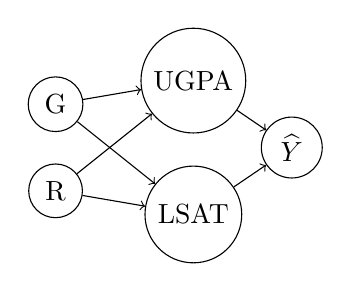
\begin{tikzpicture}
        \node (A1)  at (-1.75, -0.55) [circle, draw]{R};
        \node (A2)  at (-1.75, 0.55) [circle, draw]{G};
        \node (X1) at (0, 0.85) [circle, draw]{UGPA};
        \node (X2) at (0,-0.85) [circle,draw]{LSAT};
        \node (Y)  at (1.25, 0) [circle, draw]{$\widehat{Y}$};
        \draw[->] (A1) to (X1) {};
        \draw[->] (A1) to (X2) {};
        \draw[->] (A2) to (X1) {};
        \draw[->] (A2) to (X2) {};
        \draw[->] (X1) to (Y) {};
        % \draw[->] (X1) to (X2) {};
        \draw[->] (X2) to (Y) {};
    \end{tikzpicture}
\end{figure}
\end{minipage}
\begin{minipage}{.55\linewidth}
\begin{align*}
\mathcal{M} \, & 
\begin{cases}
    R & \leftarrow U_{R}\\
    G & \leftarrow U_G \\
    UGPA & \leftarrow b_U + \beta_1 \cdot R + \lambda_1 \cdot G + U_1, \ \\
    LSAT & \leftarrow  \exp\{b_L + \beta_2 \cdot R + \lambda_2 \cdot G + U_2\}, \\
\end{cases}
\end{align*}
\begin{align*}
    \widehat{Y} & = b(UGPA, LSAT) 
    % \\
    % & = \mathbbm{1}\{(0.6 \cdot UGPA + 0.4 \cdot LSAT) > \psi\}
\end{align*}
\end{minipage}
\caption{The auxiliary causal knowledge for Section~\ref{sec:Experiments.Real}. Let $R$ denote race, $G$ gender, \textit{LSAT} law school admissions test scores, \textit{UGPA} undergraduate grade-point average, and $\hat{Y}$ the admissions decision by $b()$.}
\label{fig:LawSchool}
% \vspace{-2ex}
\end{figure}
%

Let us now consider the law school admissions scenario popularized by \textcite[Figure 2]{Kusner2017CF}.
We use US data from the Law School Admission Council survey \parencite{Wightman1998_LawDataSource}, and recreate an admissions scenario for a top US law school. 
We consider as protected attributes an applicant's gender (\textit{G}, male/female), and race (\textit{R}, white/non-white). 
We add the ADM $b(UGPA, LSAT) = \hat{Y}$, which considers the applicant's undergraduate grade-point average (\textit{UGPA}) and law school admissions test scores (LSAT). 
If an applicant is successful, $\widehat{Y}=1$; otherwise $\widehat{Y}=0$. 
We summarize the scenario in Figure~\ref{fig:LawSchool}.
We define the ADM $b()$ using the median entry requirements for the top US law school to derive the cutoff $\psi$.\footnote{That being Yale University Law School; see \url{https://www.ilrg.com/rankings/law/index/1/asc/Accept}}
Formally, we define $b()$ as $\mathbbm{1}\{(0.6 \cdot UGPA + 0.4 \cdot LSAT) > \psi\}$.
The cutoff is the weighted sum of 60\%  in \textit{UGPA} (3.93 over 4.00), and 40\%  \textit{LSAT} (46.1 over 48), giving a total of 20.8; the maximum possible score given $b()$ is 22. 
The SCM $\mathcal{M}$ and DAG $\mathcal{G}$ follow \textcite{Kusner2017CF},
with $b_U$ and $b_L$ denoting the intercepts; $\beta_1$, $\beta_2$, $\lambda_1$, $\lambda_2$ the weights; and $U_1 \sim \mathcal{N}$ and $U_2 \sim \text{Poi}$ the probability distributions.

We study the behavior of $b()$ toward $G$ and $R$.
The dataset $\mathcal{D}$ contains $n=21790$ applicants, 43.8\% being female, 16.1\% being non-white, and 8.4\% being non-white-female.
%
Despite $b()$ being externally imposed by us for the purpose of illustrating the CST framework, under $b()$ only 0.8\% of the female applicants are successful compared to 1.5\% of the male applicants; similarly, only 0.2\% of the non-white applicants are successful compared to 2.2\% of the white applicants.
It is also the case when considering the intersectional group of non-white-females, with only 0.06\% of these applicants being admitted to law school based on $b()$ compared to the 2.25\% of white-female, non-white-male, and white-male successful applicants.
Notice that $b()$ is highly selective, with an acceptance rate of just 2.31\%, or 505 out of 21790 applicants considered.
Using DP as a fairness metric, $b()$ would still be considered unfair toward female, non-white, and non-white-female applicants.

\subsubsection{Single Discrimination}
\label{sec:Experiments.Real.Single}

%
\begin{table}[t]
\caption{Number (and \% w.r.t.~non-whites) of individual discrimination cases based on $R$ using Figure~\ref{fig:LawSchool}. Marked by * are the statistically significant cases.}
  \label{table:k-results_RACE}
  \centering
  \begin{tabular}{cccccc}
    \toprule
    Method & $k=15$ & $k=30$ & $k=50$ & $k=100$ & $k=250$\\
    \midrule
    CST w/o & 256 (7.3\%) & 309 (8.8\%) & 337 (9.6\%) & 400 (11.4\%)  & 503 (14.4\%) \\
     & 244* (6.9\%) & 301* (8.6\%) & 323* (9.2\%) & 391* (11.2\%)  & 494* (14.1\%) \\
     \midrule
    ST & 33 (0.9 \%) & 51 (1.5\%) & 61 (1.7\%) & 64 (1.8\%) & 78 (2.2\%) \\
    & 28* (0.8\%) & 28* (0.8\%) & 45* (1.3\%) & 47* (1.3\%) & 61 (1.7\%) \\
    \midrule
    CST w/ & 286 (8.2\%) & 309 (8.8\%) & 337 (9.6\%) & 400 (11.4\%)  & 503 (14.4\%)\\
    & 244* (6.9\%) & 301* (8.6\%) & 323* (9.2\%) & 391* (11.2\%)  & 494* (14.1\%) \\
    \midrule
    CF & 231 (6.6\%) & 231 (6.6\%) & 231 (6.6\%) &  231 (6.6\%) &  231 (6.6\%) \\
    & 190* (5.4\%) & 231* (6.6\%) & 231* (6.6\%) & 231* (6.6\%) & 231* (6.6\%) \\
    \bottomrule
  \end{tabular}
\end{table}
%

%
\begin{table}[t]
\caption{Number (and \% w.r.t.~females) of individual discrimination cases based on $G$ Figure~\ref{fig:LawSchool}. Marked by * are the statistically significant cases.}
  \label{table:k-results_GENDER}
  \centering
  \begin{tabular}{cccccc}
    \toprule
    Method & $k=15$ & $k=30$ & $k=50$ & $k=100$ & $k=250$\\
    \midrule
    CST w/o & 78 (0.8\%) & 120 (1.3\%) & 253 (2.7\%) & 296 (3.1\%)  & 493 (5.2\%) \\
     & 43* (0.5\%) & 88* (0.9\%) & 160* (1.7\%) & 221* (2.3\%)  & 341* (3.6\%) \\
     \midrule
    ST & 77 (0.8\%) & 101 (1.1\%) & 229 (2.4\%) & 258 (2.7\%) & 484 (5.1\%) \\
    & 57* (0.6\%) & 69* (0.7\%) & 111* (1.2\%) & 124* (1.3\%) & 366 (3.8\%) \\
    \midrule
    CST w/ & 99 (1.0\%) & 129 (1.4\%) & 267 (2.8\%) & 296 (3.1\%)  & 493 (5.2\%)\\
    & 54* (0.6\%) & 92* (0.9\%) & 160* (1.7\%) & 221* (2.3\%)  & 341* (3.6\%) \\
    \midrule
    CF & 56 (0.6\%) & 56 (0.6\%) & 56 (0.6\%) &  56 (0.6\%) &  56 (0.6\%) \\
    % & 20* (0.2\%) & 15* (0.2\%) & 30* (0.3\%) & 21* (0.2\%) & 32* (0.3\%) \\
    & 20* (0.2\%) & 15* (0.2\%) & 30* (0.3\%) & 21* (0.2\%) & 32* (0.3\%) \\
    \bottomrule
  \end{tabular}
\end{table}
%

Does $b()$ discriminate against non-white applicants? 
To answer this question using CST and CF, we generate the corresponding $\mathcal{D}^{CF}_R$ using Figure~\ref{fig:LawSchool} based in the intervention $do(R:=0)$, or \textit{what would have happened had all law school applicants been white?}
Similarly, does $b()$ discriminate against female applicants?
To answer this question using CST and CF, we generate the corresponding $\mathcal{D}^{CF}_G$ using Figure~\ref{fig:LawSchool} based in the intervention $do(G:=0)$, or \textit{what would have happened had all law school applicants been male?}
Both questions share the same $\mathcal{D}$.
Similar to Section~\ref{sec:Experiments.IllustrativeExample}, we use Definition~\ref{def:IndDisc} for detecting individual discrimination cases and Definition~\ref{def:CIs} for determining whether these cases are statistically significant.
Tables~\ref{table:k-results_RACE} and \ref{table:k-results_GENDER} show the results for all methods.
 
Tables~\ref{table:k-results_RACE} and \ref{table:k-results_GENDER} report similar patterns to those in Table~\ref{table:k-results}.
CST w/o detects a higher number of cases than ST; CST w/ detects a high number of cases than CF; and CST w/ detects a higher number than CST w/o. 
For all these patterns, though, the differences between the corresponding methods is smaller than those observed in Table~\ref{table:k-results}.
This is due to the composition of $\mathcal{D}$ and the nature of $b()$. 
Here, we work with a larger $\mathcal{D}$ (21790 versus 5000 applicants) and a more selective $b()$ (2.31\% versus 53.3\% acceptance rate).
CST w/o and CST w/ in Table~\ref{table:k-results_GENDER} converge already at larger neighborhood sizes, which does not occur in Table~\ref{table:k-results} (there is, though, a clear pattern that it occurs eventually as shown in Figure~\ref{fig:TwoCSTs_k_param}).
We also observe similar patterns once we account for statistical significance with CST w/o and CST w/ reaching the same number of cases in both tables for $k=250$.

%
\begin{figure}[t]
    \begin{subfigure}{.45\linewidth}
    \includegraphics[scale=0.45]{figures/R_all_delta_versus_k.png}
    \caption{}
     % \label{fig:a}
    \end{subfigure}
\hfill
    \begin{subfigure}{.45\linewidth}
    \includegraphics[scale=0.45]{figures/G_all_delta_versus_k.png}
    \caption{}
     % \label{fig:b}
    \end{subfigure}
\medskip
   \begin{subfigure}{.45\linewidth}
    \includegraphics[scale=0.45]{figures/R_all_nums_versus_k.png}
    \caption{}
     % \label{fig:c}
    \end{subfigure}
\hfill
    \begin{subfigure}{.45\linewidth}
    \includegraphics[scale=0.45]{figures/G_all_nums_versus_k.png}
    \caption{}
     % \label{fig:d}
    \end{subfigure}
\caption{Average $\Delta p$ and number of cases for race ($R$) and gender ($G$), respectively. We plot all and statistically significant (sig.) cases for each method.}
\label{fig:LawSchoolSingleDiscrimiantion_allmethods_k_param}
\end{figure}
%

Figure~\ref{fig:LawSchoolSingleDiscrimiantion_allmethods_k_param} supports Tables~\ref{table:k-results_RACE} and \ref{table:k-results_GENDER}, showing the average $\Delta p$ and the number of cases up to $k=500$ for all methods.\footnote{Due the size of $\mathcal{D}$, we run the methods for $k$ equals 1, 15, 30 and between 50-500 in increments of 10.} 
For the average $\Delta p$, as shown in sub-figures (a) and (b), it decreases as $k$ increases, with all methods seemingly converging to a single value.
%
% Notably, 
By observing that, as $k \rightarrow \infty$, the neighborhoods of the complainant and its counterfactual include all protected and unprotected instances, respectively, in $\mathcal{D}$, this value turns out to be the difference in DP: $P(\hat{Y}|A=1) - P(\hat{Y}|A=0)$ (cfr., footnote~\ref{foot:dp}) .
%
The average $\Delta p$ for significant cases is higher to, see ST in (a), or almost the same as, see CST w/ in (a), for all the cases.  
As $k$ increases, the control and tests groups constructed by ST, CST w/o, and CST w/ start considering new instances further away from the search centers and whatever detected initial deviation from $\tau$ dissipates slowly.
%
Similarly, as shown in sub-figures (c) and (d), the number of cases increases as $k$ increases except for CF which is independent of $k$ and its significant cases that are bounded by CF itself. 
We observe the CST versions converging, especially when accounting for statistical significance, while ST remains below both CST versions in (c) and mimics CST w/o in (d).
The number of significant cases is lower to ST in (c), or almost the same as both CST versions in (c) for all cases. 

The number of cases varies across the methods between Tables~\ref{table:k-results_RACE} and \ref{table:k-results_GENDER}. 
This is due to race and gender having different non-protected and protected search spaces.
The results are comparable, but represent separate tests for single discrimination.
Recall that non-whites represent 16.1\% while females represent 43.8\% of $\mathcal{D}$. 
It means that CST has access to a smaller search space when building the control groups for non-white complainants relative to female complainants.
Notably, in Table~\ref{table:k-results_RACE} statistically significant CF cases reach the 231 CF total cases within the $k$ values considered. 
This does not occur in Table~\ref{table:k-results_GENDER} in which the statistically significant CF cases slowly increase, though in a non-monotonically way, toward the 56 CF total cases.
Such oscillation, we believe, is due to the statistical estimator not yet reaching its asymptotic behavior.
These are, though, minor fluctuations as the number of statistically significant cases is around 0.2-0.3\%.\footnote{We use the CI \eqref{eq:CIs} from CST w/ though conditioned on CF discrimination occurring. We only detect 56 cases of CF discrimination (Table~\ref{table:k-results_GENDER}). As $k$ increases, we always look at these complainants.}
In Figure~\ref{fig:LawSchoolSingleDiscrimiantion_allmethods_k_param} we observe this non-monotonic increase for number of cases and decrease for the average $\Delta p$ of cases detected more clearly in the sub-figures (a) and (c) for race than for the sub-figures (b) and (d) for gender. 
The plots for gender are considerably less smooth than those for race. 
The composition of $\mathcal{D}$ clearly plays a role here as females represent 43.8\% and non-whites 16.1\% of the dataset, with the k-NN based methods varying more between iterations as they explore a much denser search space.

\subsubsection{Multidimensional Discrimination}
\label{sec:Experiments.Real.Multi}

We present the results for the forms of multidimensional discrimination, multiple and intersectional.
Given the focus on gender and race, the non-protected group amounts to the non-protected groups based on race and gender: i.e., white and male applicants.
As these two groups of applicants are not mutually exclusive, white-females and non-white-males are also part of the non-protected group.
This point is clearer when we consider the intersection of race and gender and focus on the protected group that is non-white-female applicants: the complementary of such group, meaning the non-protected group, includes white-female, non-white-male, and white-male applicants.

%
\begin{table}[t]
  \caption{Number (and \% w.r.t.~non-white-females) of multiple individual discrimination cases in Section~\ref{sec:Experiments.Real} for $R$ and $G$. Marked by * are the statistically significant cases.}
  \label{table:k-results_Multiple}
  \centering
  \begin{tabular}{cccccc}
    \toprule
    Method & $k=15$ & $k=30$ & $k=50$ & $k=100$ & $k=250$\\
    \midrule
    CST w/o & 8 (0.44\%) & 10 (0.55\%) & 20 (1.09\%) & 20 (1.09\%)  & 40 (2.18\%) \\
     & 4* (0.22\%) & 6* (0.33\%) & 11* (0.60\%) & 17* (0.93\%)  & 24* (1.31\%) \\
     \midrule
    ST & 5 (0.27\%) & 5 (0.27\%) & 12 (0.65\%) & 19 (1.04\%) & 24 (5.1\%) \\
    & 0* (0.0\%) & 0* (0.0\%) & 5* (0.27\%) & 5* (0.27\%)  & 15* (0.82\%) \\
    \midrule
    CST w/ & 9 (0.49\%) & 10 (0.55\%) & 21 (1.15\%) & 20 (1.09\%)  & 40 (2.18\%)\\
    & 4* (0.22\%) & 9* (0.49\%) & 11* (0.60\%) & 17* (0.93\%)  & 24* (1.31\%) \\
    \midrule
    CF & 5 (0.27\%) & 5 (0.27\%) & 5 (0.27\%) & 5 (0.27\%) & 5 (0.27\%) \\
    & 0* (0.0\%) & 3* (0.16\%) & 1* (0.05\%) & 1* (0.05\%) & 2* (0.11\%) \\
    \bottomrule
  \end{tabular}
\end{table}
%

%
\begin{table}[t]
  \caption{Number (and \% w.r.t.~non-white-females) of intersectional individual discrimination cases in Section~\ref{sec:Experiments.Real} for $R \times G$. Marked by * are the statistically significant cases.}
  \label{table:k-results_Intersectional}
  \centering
  \begin{tabular}{cccccc}
    \toprule
    Method & $k=15$ & $k=30$ & $k=50$ & $k=100$ & $k=250$\\
    \midrule
    CST w/o & 130 (7.1\%) & 138 (7.5\%) & 148 (8.1\%) & 160 (8.7\%)  & 199 (10.9\%) \\
    & 130* (7.1\%) & 138* (7.5\%) & 148* (8.1\%) & 160* (8.7\%)  & 199* (10.9\%) \\
     \midrule
    ST & 14 (0.8\%) & 14 (0.8\%) & 17 (0.9\%) & 24 (1.3\%) & 29 (1.6\%) \\
    & 14* (0.8\%) & 14* (0.8\%) & 13* (0.7\%) & 23* (1.3\%)  & 26* (1.4\%) \\
    \midrule
    CST w/ & 130 (7.1\%) & 138 (7.5\%) & 148 (8.1\%) & 160 (8.7\%)  & 199 (10.9\%) \\
    & 130* (7.1\%) & 138* (7.5\%) & 148* (8.1\%) & 160* (8.7\%)  & 199* (10.9\%) \\
    \midrule
    CF & 113 (6.2\%) & 113 (6.2\%) & 113 (6.2\%) & 113 (6.2\%) & 113 (6.2\%) \\
    & 113* (6.2\%) & 113* (6.2\%) & 113* (6.2\%) & 113* (6.2\%) & 113* (6.2\%) \\
    \bottomrule
  \end{tabular}
\end{table}
%

Following Definition~\ref{def:MultipleDisc}, we count as multiple discrimination based on race and gender when $\Delta p > \tau$ occurs separately for each of these protected attributes. 
Only those cases that are statistically significant for each protected attribute under CI \eqref{eq:CIs}---given the Bonferroni corrected $\alpha/2$---amount to statistically significant cases. 
We still rely on the generated $\mathcal{D}_R^{CF}$ and $\mathcal{D}_G^{CF}$ for the construction of the test groups and the original $\mathcal{D}$ for the construction of the control groups.
%
Does $b()$ discriminate against the none-white-female applicants as non-white \textit{and} as female applicants?
We present the results in Table~\ref{table:k-results_Multiple}. 
Figure~\ref{fig:LawSchoolMultiDiscrimination_allmethods_k_param}, as shown in sub-figures (a) and (c), further illustrates the results up to $k=500$. 
For the average $\Delta p$, we average those from cases detected separately under race and gender.

Following Definition~\ref{def:IntersectionaleDisc}, instead, we count intersectional discrimination based on race and gender when $\Delta p > \tau$ occurs for the intersection of these protected attributes. 
In practice, it means constructing the new protected attribute $R \times G$; updating $\mathcal{D}$ into $\mathcal{D}'$, such that $R \times G \in \mathcal{D}'$; and generating $\mathcal{D}'^{CF}$ given Figure~\ref{fig:LawSchool} under $do(R \times G := 0)$.
It implies a single discrimination run but under the ``new'' single attribute $R \times G$, representing the intersection of $R$ and $G$. 
Cases are statistically significant under CI \eqref{eq:CIs} based on $R \times G$.
Formally, in Figure~\ref{fig:LawSchool} we merge the $R$ and $G$ nodes into the single $R \times G$ in $\mathcal{G}$ node and do the same for the corresponding equations in $\mathcal{M}$ by interacting the dummy variables for $R$ and $G$ and re-estimating the regression weights \parencite{Wooldridge2015IntroductoryEconometrics}.
%
Does $b()$ discriminate against the none-white-female applicants?
We present the results in Table~\ref{table:k-results_Intersectional}.
Figure~\ref{fig:LawSchoolMultiDiscrimination_allmethods_k_param}, as shown in sub-figures (b) and (d), further illustrates the results up to $k=500$.

In Tables~\ref{table:k-results_Multiple} and \ref{table:k-results_Intersectional}, the three methods show similar patterns between them.
CST w/o detects more cases relative to ST (including statistically significant cases); CST w/ detects more cases than CF (including statistically significant cases); and the two CST versions converge once statistical significance is considered.
The same line of reasoning used before still applies here for understanding how CST, ST, and CF relate to each other.
The difference is that the protected group and, in turn, the non-protected group are defined by more than one protected attribute.
What is interesting in Table~\ref{table:k-results_Multiple} is that CST w/o and CST w/ converge early on for all cases, not just for those cases that are statistically significant.
We suspect these are cases that are clearly discriminatory under both race and gender, making them likely to be detected by multiple and intersectional discrimination testing.
All cases in Table~\ref{table:k-results_Intersectional} are also statistically significant for all methods.
It is due to $R \times G=1$ representing the most un-favored protected group from the combination of $R$ and $G$, which results in larger $\Delta p$'s and a complete convergence of all and statistically significant cases for all methods relative to multiple discrimination. 
Compare, e.g.,~(a) versus (b) and (c) versus (d) in Figure~\ref{fig:LawSchoolMultiDiscrimination_allmethods_k_param}. 
We discuss the last point in the next section.  

\subsubsection{On Multiple and Intersectional Discrimination}
\label{sec:Experiments.Real.Multiple_vs_Intersectional}

The results from the previous section support claims by legal scholars on the risk of not recognizing intersectional discrimination under non-discrimination law.
These claims, to the best of our knowledge, date back to \textcite{Crenshaw1989_DemarginalizingTheIntersection} and have become prominent again with the ongoing discussion around algorithmic discrimination \parencite{Xenidis2020_TunningEULaw}.
We suspect that, since multiple and intersectional discrimination share the protected group and the non-protected groups, there is a tendency to dismiss the latter as a special case of the former.
An in-depth legal discussion on the tension between multiple and intersectional discrimination is beyond this paper, but Tables~\ref{table:k-results_Multiple} and \ref{table:k-results_Intersectional} support the calls by these researchers to treat intersectional discrimination separate from multiple discrimination.

%
\begin{figure}[t]
    \begin{subfigure}{.45\linewidth}
    \includegraphics[scale=0.45]{figures/Multi_all_deltas_versus_k.png}
    \caption{}
    \end{subfigure}
\hfill
    \begin{subfigure}{.45\linewidth}
    \includegraphics[scale=0.45]{figures/Inter_all_deltas_versus_k.png}
    \caption{}
    \end{subfigure}
    \medskip
    \begin{subfigure}{.45\linewidth}
    \includegraphics[scale=0.45]{figures/Multi_all_nums_versus_k.png}
    \caption{}
     % \label{fig:c}
    \end{subfigure}
\hfill
    \begin{subfigure}{.45\linewidth}
    \includegraphics[scale=0.45]{figures/Inter_all_nums_versus_k.png}
    \caption{}
     % \label{fig:d}
    \end{subfigure}
\caption{Avg. $\Delta p$ and number of cases for multiple (left) and intersectional (right) discrimination on $R$ and $G$. We plot all and statistically significant (sig.) cases for all methods.}
\label{fig:LawSchoolMultiDiscrimination_allmethods_k_param}
\end{figure}
%

We acknowledge that, from a modeling perspective, a difference between Tables~\ref{table:k-results_Multiple} and \ref{table:k-results_Intersectional} is expected since we implement different procedures.
Under multiple discrimination we look at the intersection of two separate single discrimination testing runs, while under intersectional discrimination we look at a single discrimination run representing the intersection. 
%
The claims by legal scholars like \textcite{Crenshaw1989_DemarginalizingTheIntersection, Xenidis2020_TunningEULaw}, however, were not as apparent to us, meaning, in principle, we had no reason to expect a higher number of cases for intersectional discrimination over multiple discrimination.
%
In fact, from a probability theory perspective (read, the conjunction rule), if we had to choose a difference between the Tables~\ref{table:k-results_Multiple} and \ref{table:k-results_Intersectional}, we would have guessed the opposite, with multiple discrimination acting as an upper limit to intersectional discrimination.
Given these results, we now would add that such expectation holds from a modeling perspective if we agree that the intersection of $G$ and $R$ is not its own category. Let us discuss further.

The two modeling procedures allow to represent the case in which $R \times G$ is its own category (intersectional) and in which is just the conjunction of $R$ and $G$ (multiple).
This distinction, with legal origins as already argued \parencite{Crenshaw1989_DemarginalizingTheIntersection}, in fact materializes through the counterfactual representation of each complainant under these two discrimination testing procedures.
Under multiple discrimination, we still rely on $\mathcal{D}_R^{CF}$ and $\mathcal{D}_G^{CF}$ for running the methods separately on $R$ and $G$. 
We look at male and non-white conterfactuals separately. 
Although together they cover all the non-protected groups, they do not do so simultaneously: the complainant under this procedure would have been male or non-white, but not female-non-white.
%
Under intersectional discrimination, instead, we rely on updated factual and counterfactual datasets based on a ``new'' protected attribute $R \times G$. 
The counterfactual for a given compliant implies simultaneously the possibilities of white-male, white-female, and non-white-male, which introduces more randomness.
 
In Figure~\ref{fig:LawSchool}, arguably, the worst-off sub-group between $R$ and $G$ is the group of non-white-female applicants.
% Following the reasoning used in the previous paragraph,
The logic here is that non-white males, meaning $R=1$ and $G=0$, can always resort to their gender and white females, meaning $R=0$ and $G=1$, can always resort to their race.
Instead, non-white females have no single group within the space of $R \times G$ to resort to.
When we test for multiple discrimination we allow for these movements to occur by looking at $R$ and $G$ separately. 
This is because, by not intersecting $R$ and $G$, we do not consider the fact that the group at the intersection never has the choice to resort to a non-protected group. 
This lack of choice is what we represent when we test for intersectional discrimination by looking at $R \times G$ only.
%
The modeling problem for these forms of multidimensional discrimination requires further research with the goal of formalizing the role of the intersection and how it influences the control and test search spaces while taking into account the legal considerations discussed.

Back to Tables~\ref{table:k-results_Multiple} and \ref{table:k-results_Intersectional}, we argue that the observed difference comes from one protected attribute having a stronger influence than the other on the non-protected attributes. 
If that is the case, then testing separately for $R$ and $G$ should show individuals that are discriminated only by one of the protected attributes, which dismisses the multiple discrimination claim.
%
Table~\ref{table:MultivsInter} supports this argument. 
%
Notably, it is for this reason that lawyers discourage multiple discrimination claims and suggest that the complainant focuses on the most dominant protected attribute \parencite{Xenidis2020_TunningEULaw}.

In Table~\ref{table:MultivsInter}, given the results from the previous section, we focus on CST w/o for $k=15$ and look at individual discrimination cases detected as both multiple and intersectional discrimination.
We report the average $p_c$ and $p_t$ for $R$, $G$, and $R \times G$.
% We note that 
All multiple cases are included in the intersectional cases detected by CST w/o.
The first row shows these multiple discrimination cases. We observe that the average $p_c$ is greater than the average $p_t$, and thus the average $\Delta p > \tau$, for $R$, $G$, and $R \times G$. 
These are individual cases that suffer the negative effects of $R$ and $G$, separately and simultaneously, when applying to law school under $b()$.
The second row, instead, shows the intersectional cases only. 
For comparison, we provide the average $p_c$ and $p_t$ for these individuals' single discrimination tests for $R$ and $G$.
We observe that, on average, $R$ is the dominant protected attribute with a considerable difference in the proportion of negative outcomes between the control and test groups. 
This is not the case for $G$ where the average difference is negligible. 
Indeed, for these individuals, by looking at each protected attribute separately, we lose the multiple discrimination case.
In doing so, we also lose focus on what occurs at the intersection of $R \times G$.
The results in Table~\ref{table:MultivsInter} capture this lack of movement between protected and non-protected statuses experienced by those individuals at the bottom of the intersection of $R$ and $G$.

%
\begin{table}[t]
\caption{Avg. $p_c$ and $p_t$ for the ctr's and tst's groups of CST w/o for $k=15$.}
  \label{table:MultivsInter}
  \centering
  \begin{tabular}{ccccccc}
    \toprule
    & \multicolumn{6}{c}{Average}\\
    & $G$'s $p_c$ & $G$'s $p_t$ & $R$'s $p_c$ & $R$'s $p_t$ & $R \times G$'s $p_c$ & $R \times G$'s $p_t$\\
    \midrule
    Multi. and inter. & 0.59 & 0.33 & 0.51 & 0.00 & 0.66 & 0.00 \\
    Inter. only & 0.96 & 0.94 & 0.93 & 0.23 & 0.93 & 0.01 \\
    \bottomrule
  \end{tabular}
\end{table}
%

%
% EOS
%


\section{Discussion}
\label{sec:Discussion}
\section{Discussion}\label{Sec:GeneralDiscussion}

\subsection{Hypotheses}
\textbf{\textit{H1.}} Our results demonstrate a significant increase in trust scores across all the proposed visualizations featuring the conversational virtual agent, compared to \textbf{RUS}. This finding strongly supports the hypothesis that the presence of the virtual agent contributes to reducing discomfort and increasing acceptance during the robotic ultrasound procedure. Participants were able to ask questions, receive feedback, and feel reassured by the agent’s presence, which appears to have played a key role in fostering trust. Notably, several participants highlighted the hand animation of the virtual assistant holding the ultrasound probe, describing it as a crucial factor in building trust. This subtle yet meaningful interaction gave participants the impression that the virtual agent was aware of the ongoing procedure, making the system appear more intelligent and responsive. By simulating the action of guiding the probe, the virtual assistant conveyed a sense of human control, reducing the perceived detachment often associated with autonomous systems. This visual synchronization between the agent’s actions and the real-world procedure helped humanize the experience, further enhancing confidence in the system’s accuracy and reliability.
Moreover, the usability of the system also improved across all the proposed methods featuring the virtual agent, although significant improvements in usability were only observed with \textbf{AR-VG}. The perceived workload was also reduced in both \textbf{AR-VG} and \textbf{\revised{AV}-VG}. The agent’s conversational abilities, particularly in offering explanations and responding to patient inputs, likely reduced the cognitive burden and made the system easier to navigate.

\textbf{\textit{H2.}} Our results provide partial support for the hypothesis that reducing the visibility of the robot will reduce stress and improve acceptance. When comparing the three immersive visualization methods, \textbf{FV-VG} showed the highest RMSSD values among all conditions in both the resting and execution phases, with the smallest change between these phases. This suggests that participants experienced the least increase in stress during the procedure in the fully immersive environment, potentially due to the absence of the robot’s visual presence, which could reduce feelings of intimidation or anxiety. \add{However, the lack of statistical significance across conditions indicates that the visualization methods may primarily influence psychological perceptions—such as reduced anxiety and improved comfort—rather than inducing measurable changes in physiological stress responses. Additionally, a larger sample size may increase the power of statistical analyses and reveal trends not observed in this study.}
Participant feedback also highlighted the varied reactions to the lack of robot visibility. One participant with no prior experience in robotic procedures noted that in \textbf{FV-VG}, the environment felt like “an animated world,” allowing them to focus less on the procedure itself. This participant expressed a sense of relief and detachment from the robotic aspect, commenting that “before you realize it, the procedure is done.” This suggests that for those unfamiliar with robotic systems, full immersion may help reduce anxiety by removing any focus on the technical aspects of the procedure.
However, several participants with more experience in robotics, especially those with development experience, expressed discomfort with not being able to see the robot’s movements. These participants indicated they would prefer to observe the robot, as they were concerned about the possibility of malfunction or errors. This feedback aligns with the lower trust scores for \textbf{FV-VG}, compared to \textbf{AR-VG} and \textbf{\revised{AV}-VG}, despite the reduced physiological stress. The misalignment between the real and virtual bodies in \textbf{FV-VG}, combined with the complete absence of visual cues from the robot, likely contributed to a lower sense of control and trust in the system.
In contrast, \textbf{AR-VG}, where the robot is visible alongside the virtual agent, had the highest trust scores. This suggests that for many participants, being able to observe the robot’s actions provided reassurance and increased their trust in the system. Similarly, \textbf{\revised{AV}-VG}, where the robot was hidden but the patient’s real arm was visible, performed well in terms of trust, though slightly lower than \textbf{AR-VG}. These findings indicate that while reducing the robot’s visibility may lower stress, maintaining some visual connection to the real world, whether through the robot or the patient’s body, is crucial for building trust.

\textbf{\textit{H3.}} Our results indicate support for the hypothesis that the level of immersion influences patient workload and usability. Among the three immersive visualization methods, \textbf{AR-VG} demonstrated the highest usability and the lowest perceived workload. This supports the hypothesis that AR, by maintaining a connection to the real world, allows for greater situational awareness, which makes the system easier to navigate and reduces cognitive effort. Participants could see their surroundings and the virtual agent, making the experience more intuitive and less mentally taxing. The blend of real-world context with virtual elements likely contributed to both the higher usability and the lower workload.
\textbf{\revised{AV}-VG} also performed well in terms of both usability and workload, though slightly below \textbf{AR-VG}. The passthrough window, which allowed participants to see their real arm during the procedure, offered a partial connection to the real world while still immersing them in a virtual environment. This balance between immersion and real-world visibility may have helped reduce mental load compared to \textbf{FV-VG}, as participants were reassured by seeing part of their real body. However, the higher level of immersion compared to \textbf{AR-VG} might have slightly increased cognitive effort, resulting in a moderate workload and usability score.
In contrast, \textbf{FV-VG} demonstrated the lowest usability and the highest perceived workload among the three methods. The fully immersive environment removed all real-world visual cues, requiring participants to rely entirely on the virtual environment and the virtual agent for orientation and guidance. This complete detachment from the real world may have contributed to a sense of disorientation, which in turn negatively impacted usability and increased increased cognitive demand, as participants had to adapt to the fully virtual setting.


\subsection{Insights}


\textbf{Context-aware Communication.}
The importance of context-aware communication from the virtual agent was a key finding in this study, and it aligns with broader research in human-robot interaction~\cite{chevalier2022context}. In medical settings, patients often feel anxious or disconnected from autonomous systems due to the perceived lack of transparency and control. By embedding a conversational agent that is aware of the procedure’s stages—beginning, execution, and ending—our system ensured that patients were continuously informed and reassured. This type of communication reduces uncertainty, which is crucial in maintaining trust and comfort, as seen in other works that emphasize the role of transparency in fostering trust in autonomous systems~\cite{ososky2014determinants,pynadath2018transparency}. Context-aware systems that adjust feedback based on the current state of the procedure, as we implemented, align with research suggesting that timely, relevant communication enhances user experience and trust~\cite{lisetti2015now}. Moreover, while automating feedback can reduce patient cognitive load, it is important to avoid over-automation, as excessive automation can lead to a loss of sense of agency (SoA)~\cite{haggard2012sense,ueda2021influence} and potentially increase stress, especially in medical contexts where patient involvement is critical.

 
\textbf{Balancing Immersion and Real-World Context.}
One of the key insights from our study is the delicate balance between immersion and real-world context in patient experience during robotic ultrasound. While participants generally preferred \textbf{AR-VG} and \textbf{\revised{AV}-VG}, the stress levels were actually lower in \textbf{FV-VG}. This suggests that while a highly immersive environment can reduce physiological stress, it may also disconnect patients from critical real-world cues, such as the robot’s actions, which are crucial for maintaining trust and confidence. Research has shown that users tend to feel more comfortable when they have some level of real-world feedback, particularly in medical settings, where understanding the procedure is important for reducing anxiety~\cite{burghardt2018non,weisfeld2021dealing}. To address this, a potential future design could combine the benefits of both approaches. For instance, in a fully immersive VR environment, or even a calm, relaxing virtual setting, abstract representations of the robot’s state could be introduced. This would allow patients to enjoy the calming benefits of the VR environment while still being aware of the robot’s movements, thus providing both stress reduction and a sense of control. Such a hybrid visualization approach could balance immersion with real-world awareness, enhancing both comfort and trust in autonomous medical procedures.

\textbf{Patient-Centered Design.}
\add{This study represents a first step toward integrating conversational virtual agents and immersive visualizations into robotic ultrasound systems.}
%As a foundational exploration, it highlights the potential of these technologies to humanize robotic medical procedures and improve patient trust and comfort.
A key takeaway from this study is the importance of designing immersive visualizations with the patient’s experience at the forefront, particularly in procedures where patients remain conscious. Our findings emphasize that immersive technologies should not merely serve as technical enhancements but must also be tailored to meet the emotional and psychological needs of patients. The inclusion of a conversational virtual agent, for example, not only humanized the procedure but also helped reduce feelings of isolation and discomfort by providing constant reassurance.
A patient-centered approach can extend beyond medical robotics to other fields where human interaction with autonomous systems is critical. For example, future designs should prioritize personalization~\cite{athanasiou2014towards}, allowing systems to adapt to individual patient preferences, whether through adjusting levels of immersion, offering more or less transparency during the procedure, or tailoring communication styles to the patient’s comfort level. Additionally, systems can be designed to remember previous interactions, enabling the virtual agent to build rapport by referencing past experiences. For instance, when a patient returns for a follow-up visit, the system could greet them and mention something from the previous session, helping to create a more familiar and personalized interaction. Ultimately, this approach ensures that patients remain active participants in their own care, which is essential for fostering long-term trust and acceptance of autonomous technologies.

\subsection{Limitations}
\revised{While the study demonstrates promising results as a proof-of-concept, several limitations and trade-offs should be addressed in future work.}

First, tracking inaccuracies in \textbf{FV-VG} affected user confidence, with some participants reporting misalignment between their real and virtual bodies. This issue stems from two factors: 1) inaccurate hand tracking from the HMD, and 2) the IK solver estimating the arm pose based solely on the hand and head positions. To mitigate this, adding additional sensors to the arm could improve tracking accuracy. However, this would increase the complexity of the setup, which could negatively impact usability. \add{Additionally, these inaccuracies may have introduced biases, placing \textbf{FV-VG} at a disadvantage compared to other conditions. Caution is warranted when interpreting its results, as differences may stem from technical issues rather than the visualization method itself. Future studies should refine tracking mechanisms to ensure fair comparisons and address this imbalance.}

Second, while participants appreciated the conversational abilities of the virtual agent, some reported delays in communication, leading to uncertainty about whether their input was received. To address this, incorporating a visual indicator, such as the avatar nodding its head, or audio feedback, like the avatar quickly responding with a verbal acknowledgment such as “uh-hum,” could help reassure users that their input has been recognized. Additionally, the LLM powering the virtual agent could be further enhanced by training it on more specific data. This would enable the agent to provide more professional and accurate answers during interactions, improving the overall user experience.

Third, in the \textbf{\revised{AV}-VG} implementation, due to technical limitations, virtual elements are not visible in the passthrough window. This is because the Unity Meta Quest SDK only allows the virtual layer to be rendered either above or below the real-world layer, but not mixed. This impacts usability and overall experience, as participants felt less confident without being able to see the avatar holding the ultrasound probe. Exploring other headsets or custom rendering engines that offer more flexibility in how virtual and real-world content is layered might provide a better user experience.

Furthermore, participants noted a depth perception issue in both AR and VR visualizations. The ultrasound image attached to the probe always appeared on top of the patient’s arm, causing patients to misjudge the probe’s position. This misjudgement led to doubts about the system’s accuracy. In the future, improving the visualization of the ultrasound image—such as by adjusting its transparency when it intersects with the arm—could help resolve this issue and provide a more realistic and reassuring experience.
\add{Finally, the participant pool was skewed toward participants with prior knowledge of robotics platforms. While this demographic provided valuable insights into the usability and technical aspects of the system, it may not fully represent the target population—patients with limited exposure to robotic systems. This may have influenced the trust and acceptance measures observed in the study. Additionally, participants’ acceptance of wearing an HMD during the procedure was not separately measured but was included in overall acceptance and trust ratings for the visualizations. Another limitation is the inability to separate the effects of the virtual avatar from those of the ultrasound probe visualization. For example, trust may have increased due to the avatar, the probe visualization, or their combined effects, while usability in \textbf{VP-VG} may have been impacted by physical-virtual alignment errors. Future studies should recruit a more diverse participant pool and explore alternative methods of delivering immersive visualizations to ensure broader applicability.}

\section{Conclusion}
\label{sec:Conclusion}
%
In this work, we presented counterfactual situation testing (CST), a new actionable and meaningful framework for detecting individual discrimination in a dataset of classifier decisions.
We studied both single and multidimensional discrimination, focusing on the indirect setting.
For the latter kind, we compared its multiple and intersectional forms and provided the first evidence for the need to recognize intersectional discrimination as separate from multiple discrimination under non-discrimination law.
Compared to other methods, such as situation testing (ST) and counterfactual fairness (CF), CST uncovered more cases even when the classifier was counterfactually fair and after accounting for statistical significance.
For CF, in particular, we showed how CST equips it with confidence intervals, extending how we understand the robustness of this popular causal fairness definition. 

The decision-making settings tackled in this work are intended to showcase the CST framework and, importantly, to illustrate why it is necessary to draw a distinction between idealized and fairness given the difference comparisons when testing for individual discrimination. 
We hope the results motivate the adoption of the \textit{mutatis mutandis} manipulation over the \textit{ceteris paribus} manipulation.
We are aware that the experimental setting could be pushed further by considering higher dimensions or more complex causal structures. 
We leave this for future work.
%
Further,
extensions of CST should consider the impact of using different distance functions for measuring individual similarity \parencite{WilsonM97_HeteroDistanceFunctions}, and should explore a purely data-driven setup in which the running parameters and auxiliary causal knowledge are derived from the dataset \parencite{Cohen2013StatisticalPower, Peters2017_CausalInference}.
%
Furthermore,
extensions of CST should study settings in which the protected attribute goes beyond the binary, such as a high-cardinality categorical or an ordinal protected attribute \parencite{DBLP:journals/tkde/CerdaV22}. 
The setting in which the protected attribute is continuous is also of interest, though, in that case we could discretize it \parencite{DBLP:journals/tkde/GarciaLSLH13} and treat it as binary (the current setting) or as a high-cardinality categorical attribute.

Multidimensional discrimination testing is largely understudied \parencite{DBLP:conf/fat/0001HN23, WangRR22}. 
% Here, 
We have set a foundation for exploring the tension between multiple and intersectional discrimination, but future work should further study the problem of dealing with multiple protected attributes and their intersection.
It is of interest, for instance, formalizing the case in which one protected attribute dominates the others and the case in which the impact of each protected attribute varies based on individual characteristics.
% Formalizing the case in which one protected attribute dominates over the others as well as the case in which the effect of each protected attribute varies by individual characteristics are of interest.
While interaction terms and heterogeneous effects are understudied within SCM, both topics enjoy a well established literature in fields like economics \parencite{Wooldridge2015IntroductoryEconometrics}, which should enable future work.
% 
We hope these extensions and, overall, the fairness given the difference powering the CST framework motivate new work on algorithmic discrimination testing.

%
% EOS
%


%%
\acks{A preliminary version of this work appeared in \textcite{DBLP:conf/eaamo/AlvarezR23}. This work has received funding from the European Union’s Horizon 2020 research and innovation program under Marie Sklodowska-Curie Actions (grant agreement number 860630) for the project ``NoBIAS - Artificial Intelligence without Bias''; and from M4C2 - Investimento 1.3, Partenariato Esteso PE00000013 - ``FAIR - Future Artificial Intelligence Research'' - Spoke~1 ``Human-centered AI''. This work reflects only the authors' views and the European Research Executive Agency (REA) is not responsible for any use that may be made of the information it contains. 
We thank the three anonymous reviewers for their comments, which helped us improve considerably this work.}

%%
\appendix
%
\label{Appendix}

\section{Working Example for Generating Counterfactuals}
\label{Appendix.WorkingExampleAAP}

In this section, we present a working example to illustrate counterfactual generation. 
Given the assumptions we make for a SCM $\mathcal{M}$ \eqref{eq:SCM} in Section~\ref{sec:CausalKnowledge} and the additional assumption of an additive noise model (ANM) in Section~\ref{sec:Experiments}, such procedure is straightforward.
Suppose we have the following SCM $\mathcal{M}$ and corresponding DAG $\mathcal{G}$:

%
\begin{minipage}{.45\linewidth}
\begin{figure}[H]
\centering
    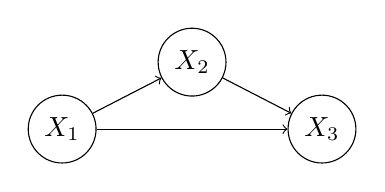
\begin{tikzpicture}
        \node (X1)  at (-1.65, 0) [circle, draw]{$X_1$};
        \node (X2) at (0, 0.85) [circle, draw]{$X_2$};
        \node (X3) at (1.65,0) [circle,draw]{$X_3$};
        % \node (Y)  at (1.75, 0) [circle, draw]{$\widehat{Y}$};
        \draw[->] (X1) to (X2) {};
        \draw[->] (X1) to (X3) {};
        % \draw[->] (X1) to (Y) {};
        \draw[->] (X2) to (X3) {};
        % \draw[->] (X2) to (Y) {};
    \end{tikzpicture}
\end{figure}
\end{minipage}
\begin{minipage}{.45\linewidth}
\begin{align*}
\mathcal{M} \, & 
\begin{cases}
    X_1 & \leftarrow U_1 \\
    X_2 & \leftarrow \alpha \cdot X_1  + U_2 \\
    X_3 & \leftarrow \beta_1 \cdot X_1 + \beta_2 \cdot X_2 + U_3
\end{cases}
\end{align*}
\end{minipage}
%

\medskip

\noindent
where $U_1, U_2, U_3$ represent the latent variables, $X_1, X_2, X_3$ the observed variables, and $\alpha, \beta_1, \beta_2$ the coefficient for the causal effect of, respectively, $X_1 \rightarrow X_2$,  $X_1 \rightarrow X_3$, and $X_2 \rightarrow X_3$. 
Suppose we want to generate the counterfactual for $X_3$, i.e., $X_3^{CF}$, had $X_1$ been equal to $x_1$. 
In the \textbf{abduction step}, we estimate $U_1$, $U_2$, and $U_3$ given the evidence, or what is observed, under the specified structural equations:
%
\begin{align*}
    \hat{U}_1 & = X_1 \\
    \hat{U}_2 & = X_2 - \alpha \cdot X_1 \\
    \hat{U}_3 & = X_3 - \beta_1 \cdot X_1 + \beta_2 \cdot X_2
\end{align*}
%
We generalize this step for \eqref{eq:SCM} as $U_j = X_j - f_j(X_{pa(j)})$ $\forall X_j \in X$. 
This step is an individual-level statement on the residual variation under SCM $\mathcal{M}$. 
It accounts for all that our assignment functions $f_j$, which are at the population level, cannot explain:~i.e., the \textit{error terms}. 
In the \textbf{action step}, we intervene $X_1$ and set all of its instances equal to $x_1$ via $do(X_1:=x_1)$ and obtain the intervened DAG $\mathcal{G}'$ and SCM $\mathcal{M}'$:

%
\begin{minipage}{.45\linewidth}
\begin{figure}[H]
\centering
    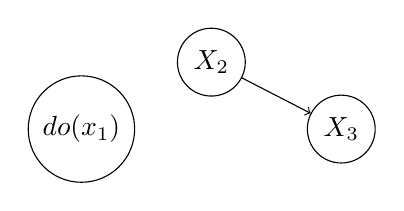
\begin{tikzpicture}
        \node (X1)  at (-1.65, 0) [circle, draw]{$do(x_1)$};
        \node (X2) at (0, 0.85) [circle, draw]{$X_2$};
        \node (X3) at (1.65,0) [circle,draw]{$X_3$};
        % \node (Y)  at (1.75, 0) [circle, draw]{$\widehat{Y}$};
        % \draw[->] (X1) to (X2) {};
        % \draw[->] (X1) to (X3) {};
        % \draw[->] (X1) to (Y) {};
        \draw[->] (X2) to (X3) {};
        % \draw[->] (X2) to (Y) {};
    \end{tikzpicture}
\end{figure}
\end{minipage}
\begin{minipage}{.45\linewidth}
\begin{align*}
\mathcal{M}' \, & 
\begin{cases}
    X_1 & = x_1 \\
    X_2 & \leftarrow \alpha \cdot x_1  + U_2 \\
    X_3 & \leftarrow \beta_1 \cdot x_1 + \beta_2 \cdot X_2 + U_3
\end{cases}
\end{align*}
\end{minipage}
%
\medskip

\noindent
where no edges come out from $X_1$ as it has been fixed to $x_1$. 
Finally, in the \textbf{prediction step}, we combine these two steps to calculate $X_3^{CF}$ under $\hat{U}$ and $\mathcal{M}'$:
%
\begin{align*}
    % X_1 &:= U_1 \\
    X_3^{CF} & \leftarrow \beta_1 \cdot x_1 + \beta_2 \cdot X_2 + \hat{U}_3 \\
             & \leftarrow \beta_1 \cdot x_1 + \beta_2 \cdot (\alpha \cdot x_1 + \hat{U}_2) + \hat{U}_3
\end{align*}
%
which is done for all instances in $X_3$. 
% This is what is done at a larger scale, for example, in \cite{Karimi2021_AlgoRecourse} and \cite{Pearl2016_CausalInference}, and also in this paper. 
The same three steps apply to $X_2$ and $X_1$.

We view the above approach as \textit{frequentist}, in particular, with regard to the abduction step.
% \footnote{This is not a formal distinction, but based on talks with other researchers. Such a distinction, to the best of our knowledge, remains an open question.} 
A more \textit{Bayesian} approach is what is done by \textcite{Kusner2017CF} in which they use a Monte Carlo Markov Chain (MCMC) to draw $\hat{U}$ by updating its prior distribution with the evidence $X$. 
In Section~\ref{sec:Experiments}, we used both approaches and found no difference in the results. 
In this work, we only present the results for the ``frequentist approach'' as it is less computationally expensive than running a MCMC. 

\section{Supplementary Material}
\label{Appendix.Supplements}

In this section, we present the supplementary material.

\subsection{Algorithms}

%
\begin{algorithm2e}[t]
\small %\scriptsize
    \caption{CST w/o $(\mathcal{D}, k, \tau, d)$}
    \label{alg:run_cfST}
	\SetKwInOut{Input}{Input}
	\SetKwInOut{Output}{Output}
	\Input{$\mathcal{D}$ - dataset, $k$ - neighborhood size, $\tau$ accepted deviation, $d$ distance function}
	\Output{$\mathcal{R}$ - set of pairs $(c, \Delta)$ of protected instance indexes and their $\Delta > \tau$}
	\BlankLine
	$\mathcal{D}_c=\{(x_i, a_i, \widehat{y}_i) \in \mathcal{D}: a_i=1\}$; \hfill\texttt{\scriptsize// control search space}\\
    $\mathcal{D}_t=\{(x_i, a_i, \widehat{y}_i) \in \mathcal{D}: a_i=0\}$\hfill\texttt{\scriptsize// test search space}\\
    $\mathcal{R} = \emptyset$\\
	\For{$(x_c, a_c, \widehat{y}_c) \in \mathcal{D}_c$}{
    $\text{\textit{k-ctr}} =
    \{ (x_i, a_i, \widehat{y}_i) \in \mathcal{D}_c: rank_{d}( x_c, x_i) \leq k \}$\hfill\texttt{\scriptsize// control group}\\
    $\text{\textit{k-tst}} = \{ (x_i, a_i, \widehat{y}_i) \in \mathcal{D}_t: rank_{d}( x^{CF}_c, x_i) \leq k \}$\hfill\texttt{\scriptsize// test group}\\
    $p_c = |\{ (x_i, a_i, \widehat{y}_i) \in \text{\textit{k-ctr}}: \hat{y}_i = 0 \}|/{k}$\hfill\texttt{\scriptsize// fraction of negative decisions for control}\\
    $p_t = |\{ (x_i, a_i, \widehat{y}_i) \in \text{\textit{k-tst}}: \hat{y}_i = 0 \}|/{k}$\hfill\texttt{\scriptsize// fraction of negative decisions for test}\\
    $\Delta = p_c - p_t$\hfill\texttt{\scriptsize// delta}\\
    \If{$\Delta > \tau$}{
    $\mathcal{R} = \mathcal{R} \cup \{(c, \Delta)\}$\hfill\texttt{\scriptsize// add pair to the result}\\
    }
	}
    \Return{$\mathcal{R}$}
\end{algorithm2e}
%

Algorithm~\ref{alg:run_cfST} reports the pseudo-code of the k-NN CST w/o algorithm. The pseudo-code is self-explanatory. 
After selecting the control and test search space (lines 1--2) as stated in Definition~\ref{def:SearchSpaces}, the algorithm iterates over the protected instances. For each of such instances, i.e., the complainant $c$, it builds (lines 5--6) the control and test groups as the $k$-nearest neighborhood instances relative to the distance $d$ for $x_c$ and for its counterfactual~$x^{CF}_c$ respectively, as stated in \eqref{eq:kctr} and \eqref{eq:ktst}. Then, the fractions $p_c$ and $p_t$ of negative decisions for the two groups are computed (lines 7--8) as stated in \eqref{eq:p1_and_p2}, as well as their difference $\Delta$ (line 9). If such a $\Delta$ is larger than the accepted deviation $\tau$, then the complainant $c$ and its $\Delta$ are added (lines 10--11) to the result $\mathcal{R}$.
%
The pseudo-code of k-NN CST w/ is a simple variant of Algorithm~\ref{alg:run_cfST}, which adds the search centers $x_c$ and $x^{CF}_c$ into the control and test groups, respectively, and divides by $k+1$ instead of $k$ at lines 7--8.

\subsection{Positive Discrimination}

Based on the discussion in Section~\ref{sec:CST_Disc}, we revisit Definitions \ref{def:IndDisc} and \ref{def:CIs} for testing individual positive discrimination under the k-NN CST. We still consider $\Delta p$ \eqref{eq:delta} and the converse of the one-sided CI $\eqref{eq:CIs}$. 

%
\begin{definition}[Positive Individual Discrimination]
\label{def:PostIndDisc}
    There is (potential) positive individual discrimination in favor of the complainant $c$ if $\Delta p < \tau$, meaning the negative decision outcomes rate for the control group is smaller than for the test group given some accepted deviation $\tau \in  [-1, 1]$.
\end{definition}
%

%
\begin{definition}[Confidence on the Positive Individual Discrimination Claim]
\label{def:PostCIs}
    A detected (potential) positive discrimination claim for the complainant $c$ by Definition~\ref{def:IndDisc}
    % by $\Delta p$ \eqref{eq:delta}  
    is statistically significant with significance level $\alpha$ if the CI $(- \infty, \Delta p + w_\alpha]$ excludes $\tau$.
\end{definition}
%

The concept of positive discrimination also applies to the case of multidimensional discrimination in Section~\ref{sec:CST.Multi}.
In that case, we would re-visit Definitions \ref{def:MultipleDisc} and \ref{def:IntersectionaleDisc} by looking at the opposite effect for $\Delta p$ across the protected attributes, be it each one of them or their intersection. 
We do not proceed with redefining these two definitions as we do not showcase them.
Again, especially for multidimensional discrimination, our focus is on discrimination \textit{against} protected groups.
Further, it is unclear what the legal scholarship views as positive multidimensional discrimination: from \textcite{Crenshaw1989_DemarginalizingTheIntersection} to \textcite{Xenidis2020_TunningEULaw}, the focus has been always on traditional discrimination.

\section{Additional Experiments}
\label{Appendix.AddExperiments}

In this section, we present additional experiments relative to the setup of Section~\ref{sec:Experiments}.

\subsection{Single Positive Discrimination}

For the same setup as in Section~\ref{sec:Experiments.SetUp} and the same data (factual and counterfactual) as in Section~\ref{sec:Experiments.IllustrativeExample}, we test for positive discrimination using Definitions \ref{def:PostIndDisc} and \ref{def:PostCIs}.
Regarding counterfactual fairness (CF), we define as positive CF discrimination when the factual has a positive decision outcome, $\hat{y}_c=1$ but its counterfactual a negative one, $\hat{y}_c^{CF}=0$.
Table~\ref{table:k-results_pos} summarizes the results for the protected attribute gender.

%
\begin{table}[t]
  \caption{Number (and \% females) of positive individual discrimination cases in Section~\ref{sec:Experiments.IllustrativeExample} based on gender. Marked by * are the statistically significant cases}
  \label{table:k-results_pos}
  \centering
  \begin{tabular}{clllll}
    \toprule
    Method & $k=15$ & $k=30$ & $k=50$ & $k=100$ & $k=250$\\
    \midrule
    CST w/o & 0 (0.0\%) & 0 (0.0\%) & 0 (0.0\%) & 0 (0.0\%)  & 0 (0.0\%) \\
     & 0* (0.0\%) & 0* (0.0\%) & 0* (0.0\%) & 0* (0.0\%)  & 0* (0.0\%) \\
     \midrule
    ST & 45 (2.6\%) & 50 (2.9\%) & 77 (4.5\%) & 118 (6.9\%) & 159 (9.3\%) \\
    & 41* (2.4\%) & 48* (2.8\%) & 55* (3.2\%) & 93* (5.4\%) & 120 (7.0\%) \\
    \midrule
    CST w/ & 0 (0.0\%) & 0 (0.0\%) & 0 (0.0\%) & 0 (0.0\%)  & 0 (0.0\%)\\
    & 0* (0.0\%) & 0* (0.0\%) & 0* (0.0\%) & 0* (0.0\%)  & 0* (0.0\%) \\
    \midrule
    CF & 0 (0.0\%) & 0 (0.0\%) & 0 (0.0\%) & 0 (0.0\%)  & 0 (0.0\%) \\
    & 0* (0.0\%) & 0* (0.0\%) & 0* (0.0\%) & 0* (0.0\%)  & 0* (0.0\%) \\
    \bottomrule
  \end{tabular}
\end{table}
%

Unlike all other single discrimination testing results in Section~\ref{sec:Experiments}, Table~\ref{table:k-results_pos} shows a ST that detects more cases than CST and a CST and CF that detect no cases at all. 
Both patterns hold when considering statistical significance.
These results are to be expected given how we generated the synthetic data for the loan application scenario. 
As described in Figure~\ref{fig:KarimiV2}, we introduced a negative systematic bias against female applicants in $\mathcal{D}$. 
This would explain why all the methods based on counterfactual generation---CF, CST w/, and CST w/o---detect zero cases: the generated male counterfactuals in $\mathcal{D}^{CF}$ can only improve over their female factual complainants in $\mathcal{D}$.
Hence, $\Delta p < \tau$ is very unlikely to occur when using CST or CF.
In other words, in a setting in which the protected individuals are always negatively affected in a systematic way, we should not expect to detect positive discrimination under methods that operationalize fairness given the difference.
Such results, for the purpose of this work, support our choice to consider only traditional discrimination as it is the most prevalent and important kind of discrimination when we suspect a negative systematic bias against the complainants. 

% Notably, 
Table~\ref{table:k-results_pos} raises questions on what kind of comparison is better suited for testing positive discrimination. 
The fact that ST, which uses an idealized comparison by implementing the CP manipulation, detects discrimination cases in a known biased setting for female applicants puts further into question the role of standard methods like it.
Is the idealized comparison suitable for positive discrimination or does \textcite{Kohler2018CausalEddie}'s criticism also apply to this setting?
Based on these preliminary results, we would argue that the tension between \textit{ceteris paribus} and \textit{mutatis mutandis} manipulations applies also to testing positive discrimination.
The stark difference between ST and CST in Table~\ref{table:k-results_pos} reinforces our view as, essentially, once we account for fairness given the difference in a known biased setting, it is difficult to argue that such a thing as positive discrimination occurs at all. 
Perhaps this is why this kind of discrimination is not discussed as much by legal scholars looking at indirect discrimination.
We plan to revisit these results in future work.

\subsection{Single Discrimination Testing}

We re-run Section~\ref{sec:Experiments.IllustrativeExample} and \ref{sec:Experiments.Real} for $\tau=0.05$, keeping all other parameters equal.
The results align with the ones we present in the main body. 
We focus on individual discrimination for all cases, not distinguishing between statistically and non-statistically significant cases.

Table~\ref{table:k-results_tau005} shows the same pattern between the CST versions relative to ST and CF as in Table~\ref{table:k-results}.
It illustrates the robustness of our framework. 
Two points we want to raise regarding Table~\ref{table:k-results_tau005}. 
First, CF, as expected, detects the same number of cases as it always looks for the strict equality between the factual and counterfactual quantities.
Second, under $\tau=0.05$, CST w/ and CST w/o align in the number of cases for larger $k$ sizes. This shows how influential $\tau$ can be for detecting discrimination, but also shows that either CST version can tackle the discrimination problem.
%
Tables \ref{table:k-results_RACE_tau005} and \ref{table:k-results_GENDER_tau005} show similar results as in, which are the $\tau=0.05$ counterparts of Tables \ref{table:k-results_RACE} and \ref{table:k-results_GENDER}. 
The results are expected given the setup. 
For both experiments the number of cases drops under $\tau=0.05$ as we have increased the difficulty of proving the individual discrimination claims.

%
\begin{table}[H]
  \caption{Number and (\% w.r.t. females) of cases based on $A$ in Figure~\ref{fig:KarimiV2}.}
  \label{table:k-results_tau005}
  \centering
  \begin{tabular}{lcccc}
    \toprule
    Method & $k=15$ & $k=30$ & $k=50$ & $k=100$ \\
    \midrule
    CST w/o & 288 (16.8\%) & 307 (17.9\%) & 331 (19.3\%) & 360 (21.0\%)  \\
    ST & 55 (3.2\%) & 60 (3.5\%) & 75 (4.4\%) & 79 (4.6\%) \\
    CST w/ & 420 (24.5\%) & 309 (18.1\%) & 334 (19.5\%) & 363 (21.2\%)  \\
    CF &  376 (22\%) &  376 (22\%) &  376 (22\%) & 376 (22\%)  \\
    \bottomrule
  \end{tabular}
\end{table}
%

%
\begin{table}[H]
  \caption{Number (and \% w.r.t.~non-whites) of cases based on $R$ using Figure~\ref{fig:LawSchool}.}
  \label{table:k-results_RACE_tau005}
  \centering
  \begin{tabular}{lccccc}
    \toprule
    Method & $k=15$ & $k=30$ & $k=50$ & $k=100$ \\
    \midrule
    CST w/o & 256 (7.30\%) & 301 (8.59\%) & 323 (9.21\%) & 376 (10.72\%)  \\
    ST & 33 (0.94\%) & 48 (1.37\%) & 57 (1.63\%) & 46 (1.31\%) \\
    CST w/ & 286 (8.16\%) & 301 (8.59\%) & 323 (9.21\%) & 376 (10.72\%)  \\
    CF &  231 (6.59\%) &  231 (6.59\%) &  231 (6.59\%) & 231 (6.59\%)  \\
    \bottomrule
  \end{tabular}
\end{table}
%
%
\begin{table}[H]
  \caption{Number (and \% w.r.t.~females) of cases based on $G$ Figure~\ref{fig:LawSchool}.}
  \label{table:k-results_GENDER_tau005}
  \centering
  \begin{tabular}{lcccc}
    \toprule
    Method & $k=15$ & $k=30$ & $k=50$ & $k=100$ \\
    \midrule
    CST w/o & 78 (0.82\%) & 105 (1.10\%) & 224 (2.35\%) & 231 (2.42\%)  \\
    ST & 77 (0.81\%) & 92 (0.96\%) & 181 (1.90\%) & 185 (1.94\%) \\
    CST w/ & 99 (1.04\%) & 105 (1.10\%) & 224 (2.35\%) & 231 (2.42\%)  \\
    CF &  56 (0.59\%) &  56 (0.59\%) &  56 (0.59\%) & 56 (0.59\%)  \\
    \bottomrule
  \end{tabular}
\end{table}
%

%
% EOS
%



% We present the relevant algorithms for the k-NN CST implementation (Section~\ref{sec:CST.AnImplementation}). The algorithm~\ref{alg:run_cfST} performs CST while algorithm~\ref{alg:get_topk} returns the indices of the top-$k$ tuples with respect to the search centers based on the distance function $d$. Notice that the main difference in algorithm~\ref{alg:run_cfST} when creating the neighborhoods is that the search centers are drawn from the factual dataset for the control group $\mathcal{D}$ and the counterfactual dataset $\mathcal{D}^{CF}$ for the test group. Further, notice that we use the same $c$ (i.e., index) for both as these two data-frames have the same structure by construction. 

% \newcommand\mycommfont[1]{\scriptsize\ttfamily\scriptsize{#1}}
% \SetCommentSty{mycommfont}

% \IncMargin{1.5em}
% \begin{algorithm2e}[h!]
% \small %\scriptsize
%     \caption{run\_CST}
%     \label{alg:run_cfST}
% 	\SetKwInOut{Input}{Input}
% 	\SetKwInOut{Output}{Output}
% 	\Input{$\mathcal{D}$, $\mathcal{D}^{CF}$, $k$}
% 	\Output{$[p_c - p_t]$}
% 	\BlankLine
% 	    $prot\_condition \leftarrow \mathcal{D}[:, \; prot\_attribute] == prot\_value$\\
% 	    $\mathcal{D}_c \leftarrow \mathcal{D}[prot\_condition]$\tcp*[f]{get protected (control) search space}\\
% 	    $\mathcal{D}_t \leftarrow \mathcal{D}[\neg \; prot\_condition]$\tcp*[f]{get non-protected (test) search space}\\
% 	    $prot\_idx \leftarrow \mathcal{D}_c.index.to\_list(\;)$\tcp*{get idx for all complainants}
% 	    $diff\_list = [ \; ]$ \\
% 	    \For{$c, \; row \in prot\_idx$}{
%         $res\_1 \leftarrow get\_top\_k(\mathcal{D}\; \; \; \; \; [c, \; :], \mathcal{D}_c, k)$\tcp*{idx of the top-k tuples for control group} 
%         $res\_2 \leftarrow get\_top\_k(\mathcal{D}^{CF}[c, \; :], \mathcal{D}_t, k)$\tcp*{idx of the top-k tuples for test group} 
%         $p_c \leftarrow sum(\mathcal{D}[res_1, \; target\_attribute]==negative\_outcome) \; / \; len(res\_1)$ \\
%         $p_t \leftarrow sum(\mathcal{D}[res_2, \; target\_attribute]==negative\_outcome) \; / \; len(res\_2)$ \\
%         $diff\_list[c] \leftarrow p_c - p_t$}
%     % \BlankLine
%     \Return{$diff\_list$}
%     % };\\ 
% \end{algorithm2e}

% \IncMargin{1.5em}
% \begin{algorithm2e}[h!]
% \small %\scriptsize
%     \caption{get\_top\_k}
%     \label{alg:get_topk}
% 	\SetKwInOut{Input}{Input}
% 	\SetKwInOut{Output}{Output}
% 	\Input{$t$, $t\_set$, $k$}
% 	\Output{$[indices]$}
% 	\BlankLine
%     % $(idx, dist) \leftarrow k\_NN(t, t\_set, k)$\tcp*{run k-NN algorithm}
%      $(idx, dist) \leftarrow k\_NN(t, t\_set, k + 1)$\tcp*{run k-NN algorithm with $k+1$}
%     \If{without search centers} {
%         $remove(t, idx, dist)$\tcp*{remove the center t from idx}
% %        \State $(idx, dist) \leftarrow k\_NN(t, t\_set, k + 1)$\tcp*{run k-NN algorithm with $k+1$}
%     }%\Else{
% %        \State $(idx, dist) \leftarrow k\_NN(t, t\_set, k)$\tcp*{run k-NN algorithm}
% %        \State $remove\_t(idx, dist)$\tcp*{remove the center t from idx}
% %    }
%     $idx' \leftarrow sort(idx, dist)$\tcp*{sort idx by the distance}
% %    \BlankLine
%     \Return{$idx'$}
%     % };\\ 
% \end{algorithm2e}




%%
\vskip 0.2in
\printbibliography
% \bibliography{references}
% \bibliographystyle{theapa}

\end{document}

%
% EOF
%
